
\documentclass[cs, msthesis]{usuthesis}

\usepackage{epsfig}
\usepackage{amssymb}           % add ams symbols stuff
\usepackage{caption}		% needed for listing captions
\usepackage{graphicx}          	% add graphics
\usepackage{subfigure}
\usepackage{color}             	% grants control of link text colors.
\usepackage[usenames,dvipsnames,rgb]{xcolor}
\usepackage{algorithm2e}
\usepackage{listings}		% code listings
\usepackage{pdflscape}
\usepackage{hyperref}          	% make contents/ref/citations clickable
\usepackage{epstopdf}
\usepackage{enumerate}		% lists of items
\usepackage{url} 			% url in bib
\usepackage{tikz}
\usetikzlibrary{decorations.text}
\usepackage{tkz-berge}
\usepackage{mathtools}
\usepackage{tabu}
\usepackage{longtable}
\usepackage{epstopdf}

% for formatting code
\lstset{
	language=C++,						% choose the language of the code
	basicstyle=\footnotesize,			% the size of the fonts that are used for the code
	numbers=left,						% where to put the line-numbers
	numberstyle=\footnotesize,			% the size of the fonts that are used for the line-numbers
	stepnumber=1,						% the step between two line-numbers. If it is 1 each line will be numbered
	firstnumber=0,
	lineskip={3pt},
	aboveskip={2\baselineskip},
	belowskip={0\baselineskip},
	xleftmargin=0mm,					% left margin of listing section
	floatplacement=t,
	numbersep=-15pt,					% how far the line-numbers are from the code
	backgroundcolor=\color{white},		% choose the background color. You must add \usepackage{color}
	showspaces=false,					% show spaces adding particular underscores
	showstringspaces=false,				% underline spaces within strings
	showtabs=false,						% show tabs within strings adding particular underscores
	frame=tb,							% adds a frame around the code
	tabsize=4,							% sets default tabsize to 2 spaces
	captionpos=b,						% sets the caption-position to bottom
	breaklines=true,					% sets automatic line breaking
	breakatwhitespace=false,			% sets if automatic breaks should only happen at whitespace
	numberbychapter=true,
	escapeinside={\%*}{*)}				% if you want to add a comment within your code
}
\lstloadlanguages{
	C++
 }

% https://tex.stackexchange.com/questions/42271/floor-and-ceiling-functions
\DeclarePairedDelimiter{\ceil}{\lceil}{\rceil}
\DeclarePairedDelimiter{\floor}{\lfloor}{\rfloor}

\newcommand*\concat{\mathbin{\|}}

\intextsep=10mm							% controls spacing before and after figures and tables
\belowcaptionskip=-5mm

%Set all linked content to be plain black text
\hypersetup{
	colorlinks,
	citecolor=black,
	filecolor=black,
	linkcolor=black,
	urlcolor=black
}


% Author and Title Information
\author{Jesse Victors}
\title{The Onion Name System: \\ Tor-powered Distributed DNS \\ for Tor Hidden Services}


% The Committee
\majorprof{Dr. Ming Li}
\firstreader{Dr. Nicholas Flann}
\secondreader{Dr. Daniel Watson}


% Graduate Dean, Update as necessary
\graddean{Dr. Mark R. McLellan}
\deantitle{Vice President for Research and}
\deansecondtitle{Dean of the School of Graduate Studies}

% Degree Information
\degree{Master of Science}
\month{May}
\year{2015}

\setcounter{tocdepth}{2}

\begin{document}

	\preliminaries   % set frontmatter style

	\maketitle
	%\makecopyright        % optional

		%

\begin{abstract}
% A space is needed before the text starts so that the first paragraph
% is indented properly.

The Tor network is a second-generation onion routing system that aims to provide anonymity, privacy, and Internet censorship resistance to its users. In recent years it has grown significantly in response to revelations of national and global electronic surveillance, and remains one of the most popular and secure anonymity network in use today. Tor is also known for its support of anonymous websites within its network. Decentralized and secure, the domain names for these services are tied to public key infrastructure (PKI) but are challenged by their long and technical addresses. In response to this difficulty, in this thesis I introduce a novel and decentralized Tor-powered DNS system that provides unique and human-meaningful domain names to Tor hidden services.

\end{abstract}

	\begin{publicabstract}
\centerline{CHAD M. MAUGHAN}
\vspace{12pt}
%Leave a blank line for formatting

Rich Web Applications (RWA) that are data driven and feature responsive user interfaces are rapidly growing in popularity.  Popular sites such as Twitter, Pandora, and Angry Birds (browser version) are all examples of popular RWAs.  These RWAs are more complex and are developed differently than many previous web sites.  More of the processing power needed to run these applications is performed on the client machine, not the server.  Due to this development strategy, testing tools need new techniques to identify web application variables, capture errors, and identify problems.  In this thesis, I introduce novel techniques to identify variables in RWA semantic URLs and automatically generate tests for RWAs using a form of testing called combinatorial testing.

\end{publicabstract}


		%

\begin{dedication}

This work is dedicated to the developers and community behind the Tor Project and the Tails OS. These individuals work tirelessly to preserve the privacy and security of everyday citizens, journalists, activists, and others around the globe, providing the much-needed service of private conversations in a very public world.

\end{dedication}
  % optional
	
%https://tex.stackexchange.com/questions/656/how-to-create-acknowledgements-in-the-report-class
\begin{dedication}

I would like to thank my major professor, Dr. Ming Li, for his continual guidance. His analysis, suggestions, and descriptions of possible attacks were instrumental in developing and solidifying this work. I would also like to extend thanks for the rest of my committee: Dr. Dan Watson and Dr. Nick Flann for their support. 

I would also like to thank Tor developers Mark Ellzey, Yawning Angel, and Nick Mathewson for their assistance with libevent and Tor technical support, Sarbajit Mukherjee for his commentary and suggestions on this work, and the Tor community for their continued support of OnioNS.

\end{dedication}     % optional
	\tableofcontents
		%\listoftables
	\listoffigures

		%\include{doc/notation}  % optional
		%\include{doc/acronyms}  % optional

	\body  % set main body style

	% Chapters
	
\chapter{INTRODUCTION}

\section{Onion Routing}

As the prevalence of the Internet and other communication has grown, so too has the development and usage of privacy-enhancing systems. These are tools and protocols that provide privacy by obfuscating the link between a user's identification or location and their communications. Privacy is not achieved in traditional Internet connections because SSL/TLS encryption cannot hide IP and TCP headers, which must be exposed to allow routing between two parties; eavesdroppers can easily break user privacy by monitoring these headers. A closely related property is anonymity -- a part of privacy where user activities cannot be tracked and their communications are indistinguishable from others. Tools that provide these systems hold a user's identity in confidence, and privacy and anonymity are often provided together. Following a general distrust of unsecured Internet communications and in light of the 2013-current revelations by Edward Snowden of Internet mass-surveillance by the NSA, GCHQ, and other members of the Five Eyes, users have increasingly turned to these tools for their own protection. Privacy-enhancing and anonymity tools may also be used by the military, researchers working in sensitive topics, journalists, law enforcement running tip lines, activists and whistleblowers, or individuals in countries with Internet censorship. These users may turn to proxies or VPNs, but these tools often track their users for liability reasons and thus rarely provide anonymity. Furthermore, they can easily voluntarily or be forced to break confidence to destroy user privacy. More complex tools are needed for a stronger guarantee of privacy and anonymity.

Today, most anonymity tools descend from mixnets, an early anonymity system invented by David Chaum in 1981.\cite{chaum2003untraceable} In a mixnet, user messages are transmitted to one or more mixes, who each partially decrypt, scramble, delay, and retransmit the messages to other mixes or to the final destination. This enhances privacy by heavily obscuring the correlation between the origin, destination, and contents of the messages. Mixnets have inspired the development of many varied mixnet-like protocols and have generated significant literature within the field of network security.\cite{edman2009anonymity}\cite{syverson2011peel}

Mixnet descendants can generally be classified into two distinct categories: high-latency and low-latency systems. High-latency networks typically delay traffic packets and are notable for their greater resistance to global adversaries who monitor communication entering and exiting the network. However, high-latency networks, due to their slow speed, are typically not suitable for common Internet activities such as web browsing, instant messaging, or the prompt transmission of email. Low-latency networks, by contrast, do not delay packets and are thus more suited for these activities, but they are more vulnerable to timing attacks from global adversaries.\cite{dingledine2004tor} In this work, we detail and introduce new functionality within low-latency protocols.

Onion routing is a technique for enhancing privacy of TCP-based communication across a network and is the most popular low-latency descendant of mixnets in use today. It was first designed by the U.S. Naval Research Laboratory in 1997 for military applications\cite{syverson1997anonymous}\cite{reed1998anonymous} but has since seen widespread usage. In onion routing with public key infrastructure (PKI), a user selects a set network nodes, typically called \emph{onion routers} and together a \emph{circuit}, and encrypts the message with the public key of each router. Each encryption layer contains the next destination for the message -- the last layer contains the message's final destination. As the \emph{cell} containing the message travels through the network, each of these onion routers in turn decrypt their encryption layer like an onion, exposing their share of the routing information. The final recipient receives the message from the last router, but is never exposed to the message's source.\cite{syverson2011peel} The sender therefore has privacy because the recipient does not know the sender's location, and the sender has anonymity if no identifiable or distinguishing information is included in their message.

\begin{figure}[htbp]
	\centering
	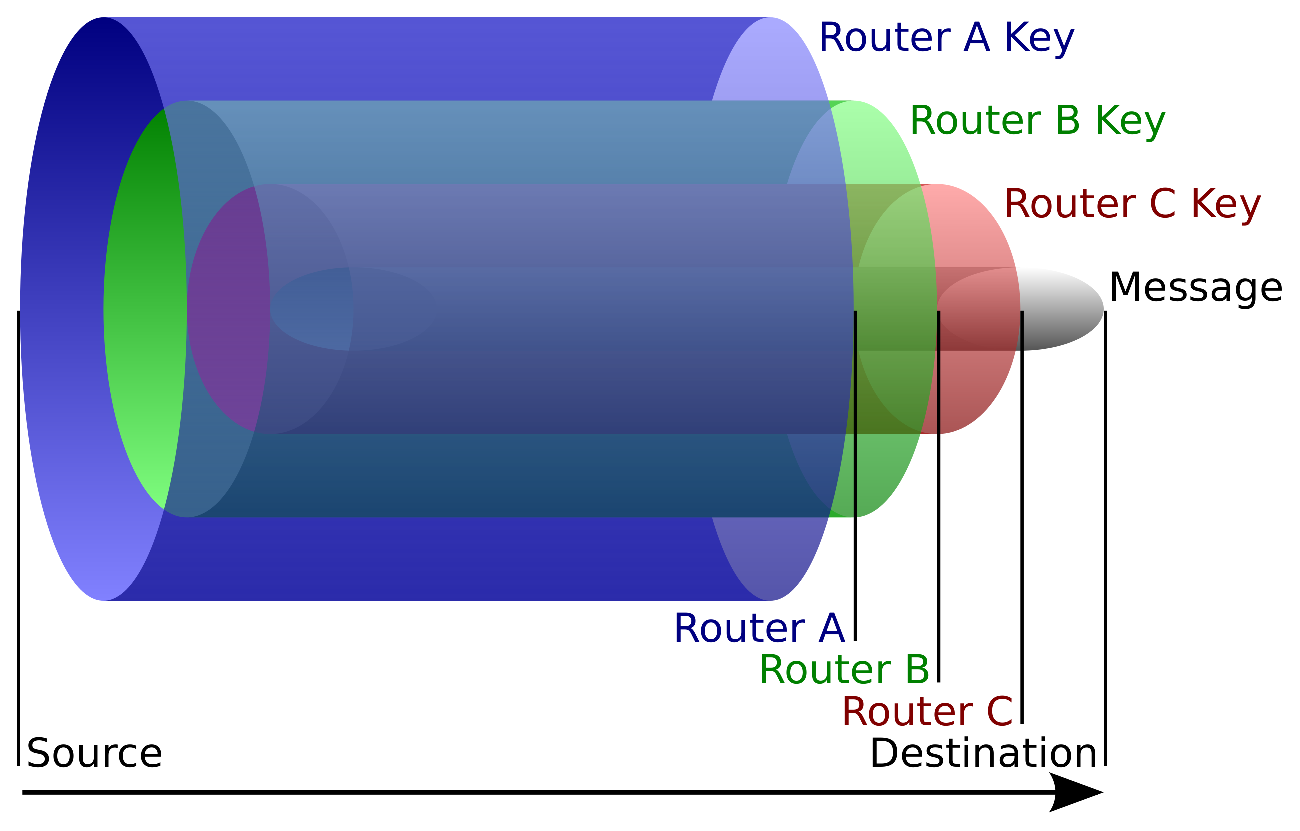
\includegraphics[width=0.5\textwidth]{images/onion-diagram.eps}
	\caption{An example cell and message encryption in an onion routing scheme. Each router ``peals'' off its respective layer of encryption; the final router exposes the final destination.}
\end{figure}

The first generation of onion routing used circuits fixed to a length of five, assumed a static network topology, and most notably, introduced the ability to mate two circuits at a common router or server. This last capability enabled broader anonymity where the circuit users were anonymous to each other and to the common server, a capability that was adopted and refined by later generation onion routers. Second generation introduced variable-length circuits, multiplexing of all user traffic over circuits, exit policies for the final router, and assumed a dynamic network by routing updates throughout the network. A client, Alice, in second-generation onion routers also distributed symmetric keys through the cell layers. If routers remember the destinations for each message they received, the recipient Bob can send his reply backwards through the circuit and each router re-encrypts the reply with their symmetric key. Alice unwraps all the layers, exposing the Bob's reply. The transition from public-key cryptography to symmetric-key encryption significantly reduced the CPU load on onion routers and enabled them to transfer more packets in the same amount of time. However, while influential, first and second generation onion routing networks have fallen out of use in favor of third-generation systems.\cite{syverson2011peel}

\section{Tor}

Tor is a third-generation onion routing system. It was invented in 2002 by Roger Dingledine, Nick Mathewson, and Paul Syverson of the Free Haven Project and the U.S. Naval Research Laboratory\cite{dingledine2004tor} and is the most popular onion router in use today. Tor inherited many of the concepts pioneered by earlier onion routers and implemented several key changes:\cite{syverson2011peel}\cite{dingledine2004tor}

\begin{itemize}
	\item \textbf{Perfect forward secrecy:} Rather than distributing keys via onion layers, Tor clients negotiate ephemeral symmetric encryption keys with each of the routers in turn, extending the circuit one router at a time. These keys are then purged when the circuit is torn down; this achieves perfect forward secrecy, a property that ensures that the session encryption keys will not be revealed if long-term public keys are later compromised.
	\item \textbf{Circuit isolation:} Second-generation onion routers mixed cells from different circuits in realtime, but later research could not justify this as an effective defence against an active adversary.\cite{syverson2011peel} Tor abandoned this in favor of isolating circuits from each other inside the network, although it recycles TCP/IP links between routers.
	\item \textbf{Three-hop circuits:} Previous onion routers used long circuits to provide heavy traffic mixing. Tor removed mixing and fell back to using short circuits of minimal length. With three relays involved in each circuit, the first router (the \emph{guard}) is exposed to the user's IP address. The middle router passes onion cells between the guard and the final router (the \emph{exit}) and its encryption layer exposes it to neither the user's IP nor its traffic. The exit processes user traffic, but is unaware of the origin of the requests. While the choice of middle and exits can be routers can be safely random, the guard must be chosen once and then consistently used to avoid a large cumulative chance of leaking the user's IP to an attacker. This is of particular importance for circuits from hidden services.\cite{bauer2007low}\cite{overlier2006locating}
	\item \textbf{Standardized to SOCKS proxy:} Tor simplified the multiplexing pipeline by transitioning from application-level proxies (HTTP, FTP, email, etc) to a TCP-level SOCKS proxy, which multiplexed user traffic and DNS requests through the onion circuit regardless of any higher protocol. The disadvantage to this approach is that Tor's client software has less capability to cache data and strip identifiable information out of a protocol. The countermeasure was the Tor Browser, a fork of Mozilla's open-source Firefox with a focus on security and privacy. To reduce the risks of users breaking their privacy through Javascript, it ships with the NoScript extension which blocks all web scripts not explicitly whitelisted. The browser also forces all web traffic, including DNS requests, through the Tor SOCKS proxy, provides a Windows-Firefox user agent regardless of the native platform, and includes many sanitization, security, and privacy enhancements not included in native Firefox. The browser also utilizes the Electronic Frontier Foundation's HTTPS Everywhere extension to re-write HTTP web requests into HTTPS whenever possible, providing an additional encryption layer that hides web traffic from exit routers.
	\item \textbf{Directory servers:} Tor introduced a set of trusted directory servers, called directory authorities, to collect, digitally sign, and distribute network information such as the IP addresses and public keys of onion routers. Onion routers mirror the network information from the directories, distributing the bandwidth load. This simplified approach is more flexible and scales faster than the previous flooding approach, but relies on the trust of central directory authorities. Tor ensures that each authority is independently maintained in multiple locations and jurisdictions, reducing the likelihood of an attacker compromising all of them.\cite{syverson2011peel} We describe the contents and format of this network information in section \ref{sec:ConsensusDocs}.
	\item \textbf{Dynamic rendezvous with hidden services:} In previous onion routers, circuits mated at a fixed common node and did not use perfect forward secrecy. Tor introduced a distributed hashtable to record the location of the introduction node for a given hidden service. Following the initial handshake, the server and the client then meet at a different onion router chosen by the client. This approach significantly increased the reliability of hidden services and distributed the communication load across multiple rendezvous points.\cite{dingledine2004tor} We provide additional details on the hidden service protocol in section \ref{sec:HiddenServices} and our motivation for addition infrastructure in section \ref{sec:Motivation}.
\end{itemize}

As of March 2015, Tor has 2.3 million daily users that together generate 65 Gbit/s of traffic. Tor's network consists of nine directory authorities and 6,600 onion routers in 83 countries.\cite{TorMetrics} In a 2012 Top Secret U.S. National Security Agency presentation leaked by Edward Snowden, Tor was recognized as the "the king of high secure, low latency Internet anonymity".\cite{landau2014highlights}\cite{plak2014anonymous} In 2014, BusinessWeek claimed that Tor was ``perhaps the most effective means of defeating the online surveillance efforts of intelligence agencies around the world.''\cite{TorBusinessWeek}

\subsection{Design}

Tor's design focuses on being easily deployable, flexible, and well-understood. Tor also places emphasis on usability in order to attract more users; more user activity translates to an increased difficulty of isolating and breaking the privacy of any single individual. Tor however does not manipulate any application-level protocols nor does it make any attempt to defend against global attackers. Instead, its threat model assumes that the capabilities of adversaries are limited to observing fractions of Tor traffic, that they can actively delay, delete, or manipulate traffic, that they may attempt to digitally fingerprint packets, that they may run onion routers themselves, and that they may compromise a fraction of other existing routers. Together, most of the assumptions may be broadly classified as traffic analysis attacks. Tor's final focus is defending against these types of attacks.\cite{dingledine2004tor}

\subsection{Circuit Construction}

\begin{figure}[htdp]
	\begin{minipage}[b]{0.48\linewidth}
		\centering
		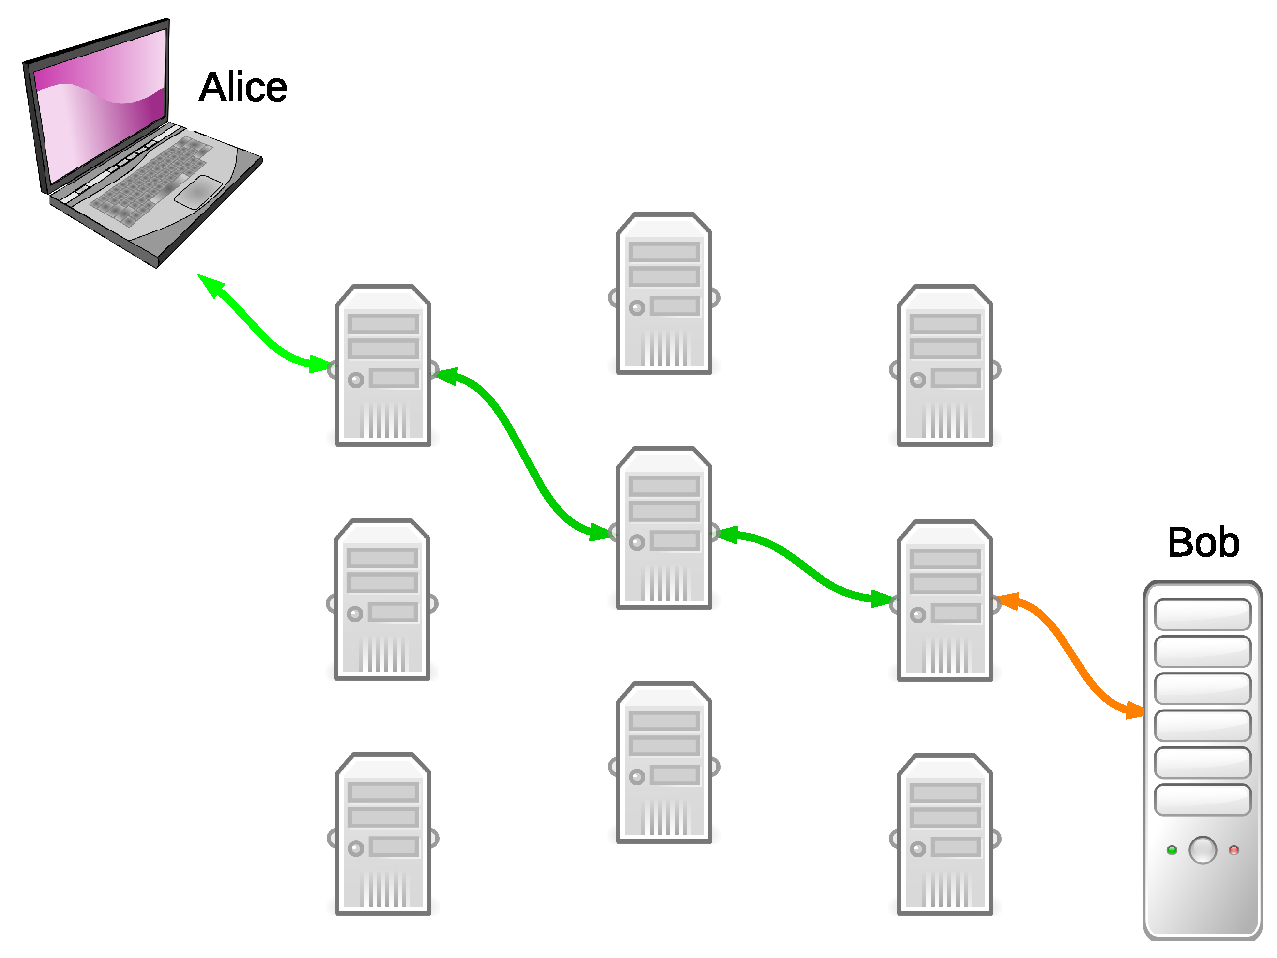
\includegraphics[width=\textwidth]{images/LucidCharts/Tor_Circuit_Orig.pdf}
	\end{minipage}
	\hspace{0.5cm}
	\begin{minipage}[b]{0.48\linewidth}
		\centering
		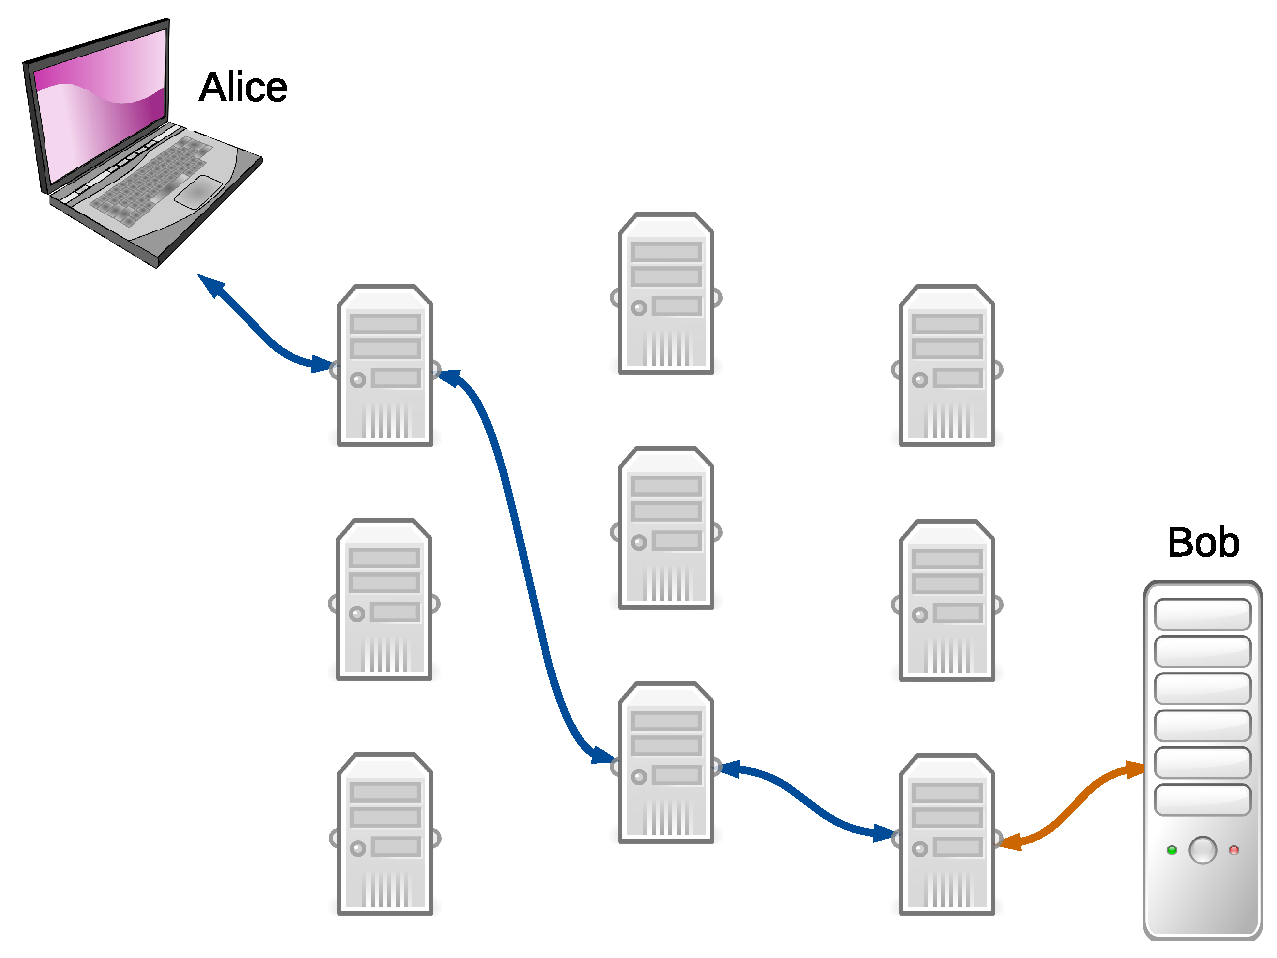
\includegraphics[width=\textwidth]{images/LucidCharts/Tor_Circuit_Change.pdf}
	\end{minipage}
	\caption{Alice communicates privately to Bob through a Tor circuit. Her communication path consists of three routers, an entry, middle, and exit. Although Bob's identity and location is known to Alice, the Tor circuit prevents Bob from knowing Alice's identity or location. At a later time, Alice may construct a different circuit to Bob, giving her a new identity from Bob's perspective. Each encrypted Tor link is shown in green, the final connection from the exit to Bob, shown in orange, is optionally encrypted.}
	\label{fig:torOverview}
\end{figure}

\subsubsection{Overview}

Let Alice be a client who wishes to enhance her privacy by using Tor but does not run a Tor router herself. Her basic procedure for initializing her own circuit is as follows:

\begin{enumerate}
	\item Alice selects a Tor router $ R_{1} $ and sets up an authenticated encrypted connection to it.
	\item Alice selects a second router $ R_{2} $ and tells $ R_{1} $ to build a TCP link to it. 
	\item Alice uses her $ R_{1} $ tunnel to establish an authenticated encrypted connection with $ R_{2} $.
	\item Alice selects an $ R_{3} $ and uses the $ Alice \leftrightarrow R_{1} \leftrightarrow R_{2} $ tunnel to tell $ R_{2} $ to connect to $ R_{3} $.
	\item Alice establishes an authenticates encrypted connection with $ R_{3} $ over the \\ $ Alice \leftrightarrow R_{1} \leftrightarrow R_{2} $ tunnel.
\end{enumerate}

Following the successful circuit construction, she can then send messages out of $ R_{3} $ through the $ Alice \leftrightarrow R_{1} \leftrightarrow R_{2} \leftrightarrow R_{3} $ tunnel. As a defence against traffic analysis, her message is padded into equally-sized Tor \emph{cells} as it travels through the network.\cite{mccoy2008shining}

\subsubsection{TAP}

The Tor Authentication Protocol (TAP) is a central exchange in Tor's networking infrastructure. If a Tor router $ R_{i} $ is known to Alice, TAP allows Alice to authenticate $ R_{i} $ and to enables them to negotiate an ephemeral session encryption key while preserving Alice's anonymity. TAP thus provides perfect forward secrecy in Tor circuits and defends against spoofing attacks.

First, TAP assumes that the following is established:

\begin{itemize}
	\item Alice has a reliable PKI that can securely distribute the identity, IP addresses, and public keys of all Tor routers. Tor accomplishes this through consensus documents from directory authorities, described in section \ref{sec:ConsensusDocs}.
	\item Let $ \mathcal{E}_{B} $ mean encryption and $ \mathcal{D}_{B} $ mean decryption under $ B $'s public-private keypair for some party $ B $.
	\item $ p $ is a prime such that $ q = \frac{q - 1}{2} $ is also prime and let $ g $ be a generator of the subgroup of $ \mathbb{Z}^{*}_{p} $ of order $ q $.
	\item Let $ R_{L} $ be a generator that returns uniformly random $ L $-bit values in the interval $ [1, \textrm{min}(q, 2 ^ L) - 1] $.
	\item Define $ f $ as SHA-1 which takes input from $ \mathbb{Z}_{p} $ and returns a $ L_{f} $-bit value.
\end{itemize}

Then TAP proceeds as:

\begin{enumerate}
	\item \label{item:First1}
		\begin{enumerate}
			\item Alice selects a Tor router, $ R_{i} $.
			\item Alice generates $ x = R_{L} $ and computes $ s = g ^ x \bmod{p} $.
			\item Alice sends $ c = \mathcal{E}_{R_{i}}(s) $ to $ R_{i} $.
		\end{enumerate}
	\item
		\begin{enumerate}
			\item $ R_{i} $ computes $ m = \mathcal{D}_{R_{i}}(c) $ and confirms that $ 1 < m < p - 1 $.
			\item $ R_{i} $ generates $ y = R_{L} $ and computes $ a = g ^ y \bmod{p} $ and $ b = f(m ^ y \bmod{p}) $.
			\item $ R_{i} $ sends $ (a, b) $ to Alice.
		\end{enumerate}
	\item
		Alice confirms that $ 1 < a < p - 1 $ and that $ b = f(a ^ x \bmod{p}) $.
	\item \label{item:Last1}
		If the assertions pass, then Alice has confirmed $ R_{i} $'s identity and now Alice and $ R_{i} $ can use $ a ^ x = m ^ y $ as a shared symmetric encryption key and encrypt messages under AES.
	\item 
		Alice repeats steps \ref{item:First1} -- \ref{item:Last1} until the circuit is of the desired length.
\end{enumerate}

\begin{figure}[htbp]
	\centering
	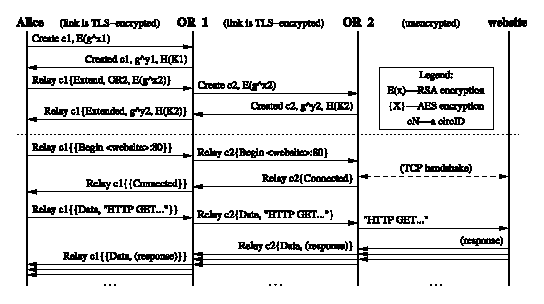
\includegraphics[width=0.9\textwidth]{images/Tor/tap.eps}
	\caption{The Tor Authentication Protocol negotiated over two onion routers. Following circuit construction, Alice sends a HTTP request to the target server, which is encrypted by each router as it travels back up the circuit.\cite{dingledine2004tor}\cite{ling2013protocol}}
\end{figure}

Thus for each router in the circuit, Alice perform one public-key encryption and her half of a Diffie-Hellman-Merkle (DHE) handshake, and each router in turn performs one private-key decryption and their half of a DHE handshake. Under the assumptions that RSA is one way, AES remains unbroken, and $ f $ is strong and acts as a random oracle, an attacker has only a negligible chance of being able to impersonate $ R_{i} $ and read messages that she tunnels through the circuit.\cite{goldberg2006security}

\subsubsection{NTor}

In mid 2013, TAP was superseded by NTor, a new protocol invented by Goldberg, Stebila, and Ustaoglu.\cite{goldberg2013anonymity} Compared to TAP, NTor replaced the computational cost associated with DHE exponentiation with significantly more efficient elliptic curve cryptography (ECC). Its implementation uses Curve25519,\cite{bernstein2006curve25519} a Montgomery curve designed by Bernstein for high-speed ECDHE key exchanges. All Curve25519 operations are implemented to run in $ \mathcal{O}(1) $ time.

NTor is initialized by defining the following,

\begin{itemize}
	\item Let $ H(x,k) $ be HMAC-SHA256, which accepts a message $ x $ and yield a 32-byte MAC output. Let $ k_{1} $, $ k_{2} $, and $ k_{3} $ be some fixed secret keys for the HMAC algorithm, $ k_{1} \neq k_{2} \neq k_{3} $.
	\item Let $ \mathit{C}_{\mathit{gen}}() $ generate a Curve25519 keypair. This function requires 32 bytes from a cryptographically secure source (such as a CSPRNG) to generate the private key, then it derives the public key.
	\item Let $ \mathit{C}_{\mathit{sec}}(pvt, pub) $ yield a 32-byte common secret given a Curve25519 private and public key, $ pvt $ and $ pub $, respectively.
	\item Let each Tor router $ R_{j} $ generate $ b_{j},B_{j} = \mathit{C}_{\mathit{gen}}() $ and publish $ B_{j} $ through the consensus document.
	\item Let $ \mathit{id} $ by the router's identification fingerprint.
\end{itemize}

Then NTor proceeds as:

\begin{enumerate} % 216-ntor-handshake.txt
	\item \label{item:First2}
		\begin{enumerate}
			\item Alice selects a Tor router, $ R_{i} $.
			\item Alice generates $ x,X = C_{\mathit{gen}}() $ and sends $ X $ to $ R_{i} $.
		\end{enumerate}
	\item
		\begin{enumerate}
			\item $ R_{i} $ generates $ y,Y = C_{\mathit{gen}}() $.
			\item $ R_{i} $ sets $ \mathit{sec} = C_{\mathit{sec}}(y, X) \concat C_{\mathit{sec}}(b, X) \concat \mathit{id} \concat X \concat Y $.
			\item $ R_{i} $ computes $ \mathit{seed} = H(\mathit{sec, k_{1}}) $.
			\item $ R_{i} $ computes $ \mathit{auth} = H(H(\mathit{sec, k_{2}}) \concat id \concat B \concat Y \concat X, k_{3}) $.
			\item $ R_{i} $ sends $ Y $ and $ \mathit{auth} $ to Alice.
			\item $ R_{i} $ deletes the $ y,Y $ keypair.
		\end{enumerate}
	\item
		\begin{enumerate}
			\item Alice sets $ \mathit{sec} = C_{\mathit{sec}}(x, Y) \concat C_{\mathit{sec}}(x, B) \concat \mathit{id} \concat X \concat Y $.
			\item Alice computes $ \mathit{seed} = H(\mathit{sec, k_{1}}) $.
			\item Alice confirms that $ \mathit{auth} = H(H(\mathit{sec, k_{2}}) \concat id \concat B \concat Y \concat X, k_{3}) $.
		\end{enumerate}
	\item
		Alice and $ R_{i} $ now have a shared secret $ \mathit{seed} $ that is then used indirectly for symmetric key encryption.	
\end{enumerate}

\subsection{Consensus Documents}
\label{sec:ConsensusDocs}

As previously mentioned, early mixnets and onion routers either assumed a static network topology or flooded updates across the network. By contrast, Tor's network is maintained by a small set of semi-trusted directory authorities. Periodically, Tor routers upload digitally signed ``descriptors'' to these authorities. A descriptor may contain essential routing numbers, router capabilities, cryptographic keys, bandwidth history, or other information.

Each directory authority maintains an long-term authority key (distinct from its normal identity key if it is a Tor router) and a medium-term signing key. Periodically, each directory authority 

\begin{enumerate}
	\item Aggregates the descriptors into a single ``status vote'' document.
	\item Signs its vote with its signing key.
	\item Exchanges its vote and signature with all other authorities.
	\item Computes a single network status consensus from all the other voting documents.
	\item Signs the network consensus and exchanges the signature with all other authorities.
\end{enumerate}

Once this is complete, the consensus is published and is available for download. If clients have knowledge of the Tor network, they may download the more recent consensus from the directory-mirroring routers. By this system, new routers or changes to existing routers can be propagated to all parties within a very short timeframe. Although routers can optionally publish additional non-essential descriptors, clients and routers typically only need the essential descriptors containing routing information, directory signing keys, and router keys. We discuss the documents containing these descriptors below:\cite{TorCollector}\cite{TorDirSpec}

\subsubsection{cached-certs}

The \emph{cached-certs} document contains the long-term authority identity keys and the medium-term signing keys from each directory authority. The Tor source includes the long-term keys, so all parties can verify the authenticity of the signing keys and in turn the descriptors signed by them. They will believe router descriptors if more than half of the authorities have signed it. Each certificate contains the following fields:

\begin{itemize}
	\item \textbf{fingerprint:} The SHA-1 hash of the identity key.
	\item \textbf{dir-key-published:} The time in UTC when the keys were last published.
	\item \textbf{dir-key-expires:} The time in UTC when the signing keys expire.
	\item \textbf{dir-identity-key:} The identity key, typically a 3072-bit RSA key.
	\item \textbf{dir-signing-key:} The signing key, typically a 2048-bit RSA key.
	\item \textbf{dir-key-crosscert:} The signature of the identity key, made using the signing key.
	\item \textbf{dir-key-certification:} The signature of the above fields, made using the identity key.	
\end{itemize}

\subsubsection{cached-microdesc-consensus}

The \emph{cached-microdesc-consensus} document contains network status information. The document includes a header and then a list of condensed descriptors from each router, called microdescriptors. The header includes the following fields:

\begin{itemize}
	\item \textbf{valid-after} (VA), \textbf{fresh-until} (FU), and \textbf{valid-until} (VU). Three timestamps in UTC, $ \mathrm{VA} < \mathrm{FU} < \mathrm{VU} $. VA and VU specifies the earliest and latest time that these descriptors are valid, respectively. All three values are chosen such that two consensuses overlap: $ \mathrm{consensus}_{x} $ will be considered fresh until $ \mathrm{consensus}_{x+1} $ becomes valid, and then $ \mathrm{consensus}_{x} $ expires when $ \mathrm{consensus}_{x+1} $ is no longer fresh.
	\item \textbf{client-versions} and \textbf{server-versions:} An ascending list of recommended Tor versions for clients and routers, respectively.
	\item A list of directory authorities, each containing:
		\begin{itemize}
			\item \textbf{dir-source:} The authority's nickname, fingerprint, IP address, onion routing port, and directory port.
			\item \textbf{contact:} Optional contact information for the authority operator.
			\item \textbf{vote-digest:} The hash of the authority's status vote document.
		\end{itemize}
\end{itemize}

Following the header, each microdescriptor contains:

\begin{itemize}
	\item \textbf{r:} The router's nickname, fingerprint, time of last restart, IP address, onion routing port, and directory port.
	\item \textbf{m:} The SHA-256 hash of the router's microdescriptor. This also includes its entries in the \emph{cached-microdescs} document (discussed below).
	\item \textbf{s:} A list of the router's status flags, as given by the directory authorities. Common examples include Running, Valid, Fast, Guard, Stable, and Exit.
	\item \textbf{v:} The version of the Tor software that the router is running, as reported by the router.
	\item \textbf{w:} The estimated bandwidth that this router is capable of. This value is determined by speed tests from bandwidth authorities, who are a subset of the directory authorities.
\end{itemize}

\subsubsection{cached-microdescs}

The \emph{cached-microdescs} document contains cryptographic keys from each Tor router. Each entry contains:

\begin{itemize}
	\item \textbf{onion-key:} The router's public RSA key, primarily used for TAP authentication.
	\item \textbf{ntor-onion-key:} The router's public Curve25519 key, primarily used for NTor.
	\item \textbf{family:} The fingerprint of routers also under the operator's administration; Tor clients will not construct circuits through any routers that have the same family or that are in the same /16 IPv4 block.
	\item \textbf{id:} The router's fingerprint.
\end{itemize}

\subsection{Hidden Services}
\label{sec:HiddenServices}

Although Tor's primary and most popular use is for secure access to the traditional Internet, Tor also supports \emph{hidden services} -- anonymous servers hosting services such as websites, marketplaces, or chatrooms. These servers intentionally mask their IP addresses through Tor circuits and thus cannot normally be accessed outside the context of Tor. In contrast to Tor-anonymized web requests where the client is anonymous but the server is known, Tor hidden services provide bidirectional anonymity where both parties remain anonymous and never directly communicate with one another.\cite{nicolussi2011human}

Tor does not contain a DNS system for its websites; instead hidden service addresses are algorithmically generated by generating the SHA-1 hash of their public RSA key, truncating to 80 bits, and converting the remainder to base58. Ignoring the possibility of SHA-1 collisions, this builds a one-to-one relationship between a hidden service's public key and its address which can be confirmed without requiring any identifiable information or central authorities. The address is the appended with the .onion Top-Level Domain (TLD).

A hidden server, Bob, first builds Tor circuits to several random relays and enables them to act as \textit{introduction points} by giving them its public key, $ B_{K} $. He then then uploads his public key and the fingerprint identity of these nodes to a distributed hashtable inside the Tor network, signing the result. He then publishes his hidden service address in a backchannel. When Alice obtains this address and enters it into a Tor-enabled browser, her software queries this hashtable, obtains $ B_{K} $ and Bob's introduction points, and builds a Tor circuit to one of them, $ ip_{1} $. Simultaneously, the client also builds a circuit to another relay, $ rp $, which she enables as a rendezvous point by telling it a one-time secret, $ sec $. During this procedure, hidden services must continue to use their same entry node in order to avoid leaking its IP address to possibly malicious onion routers.\cite{bauer2007low}\cite{overlier2006locating}

%\begin{figure}[htdp]
%	\begin{minipage}[b]{0.45\linewidth}
%		\centering
%		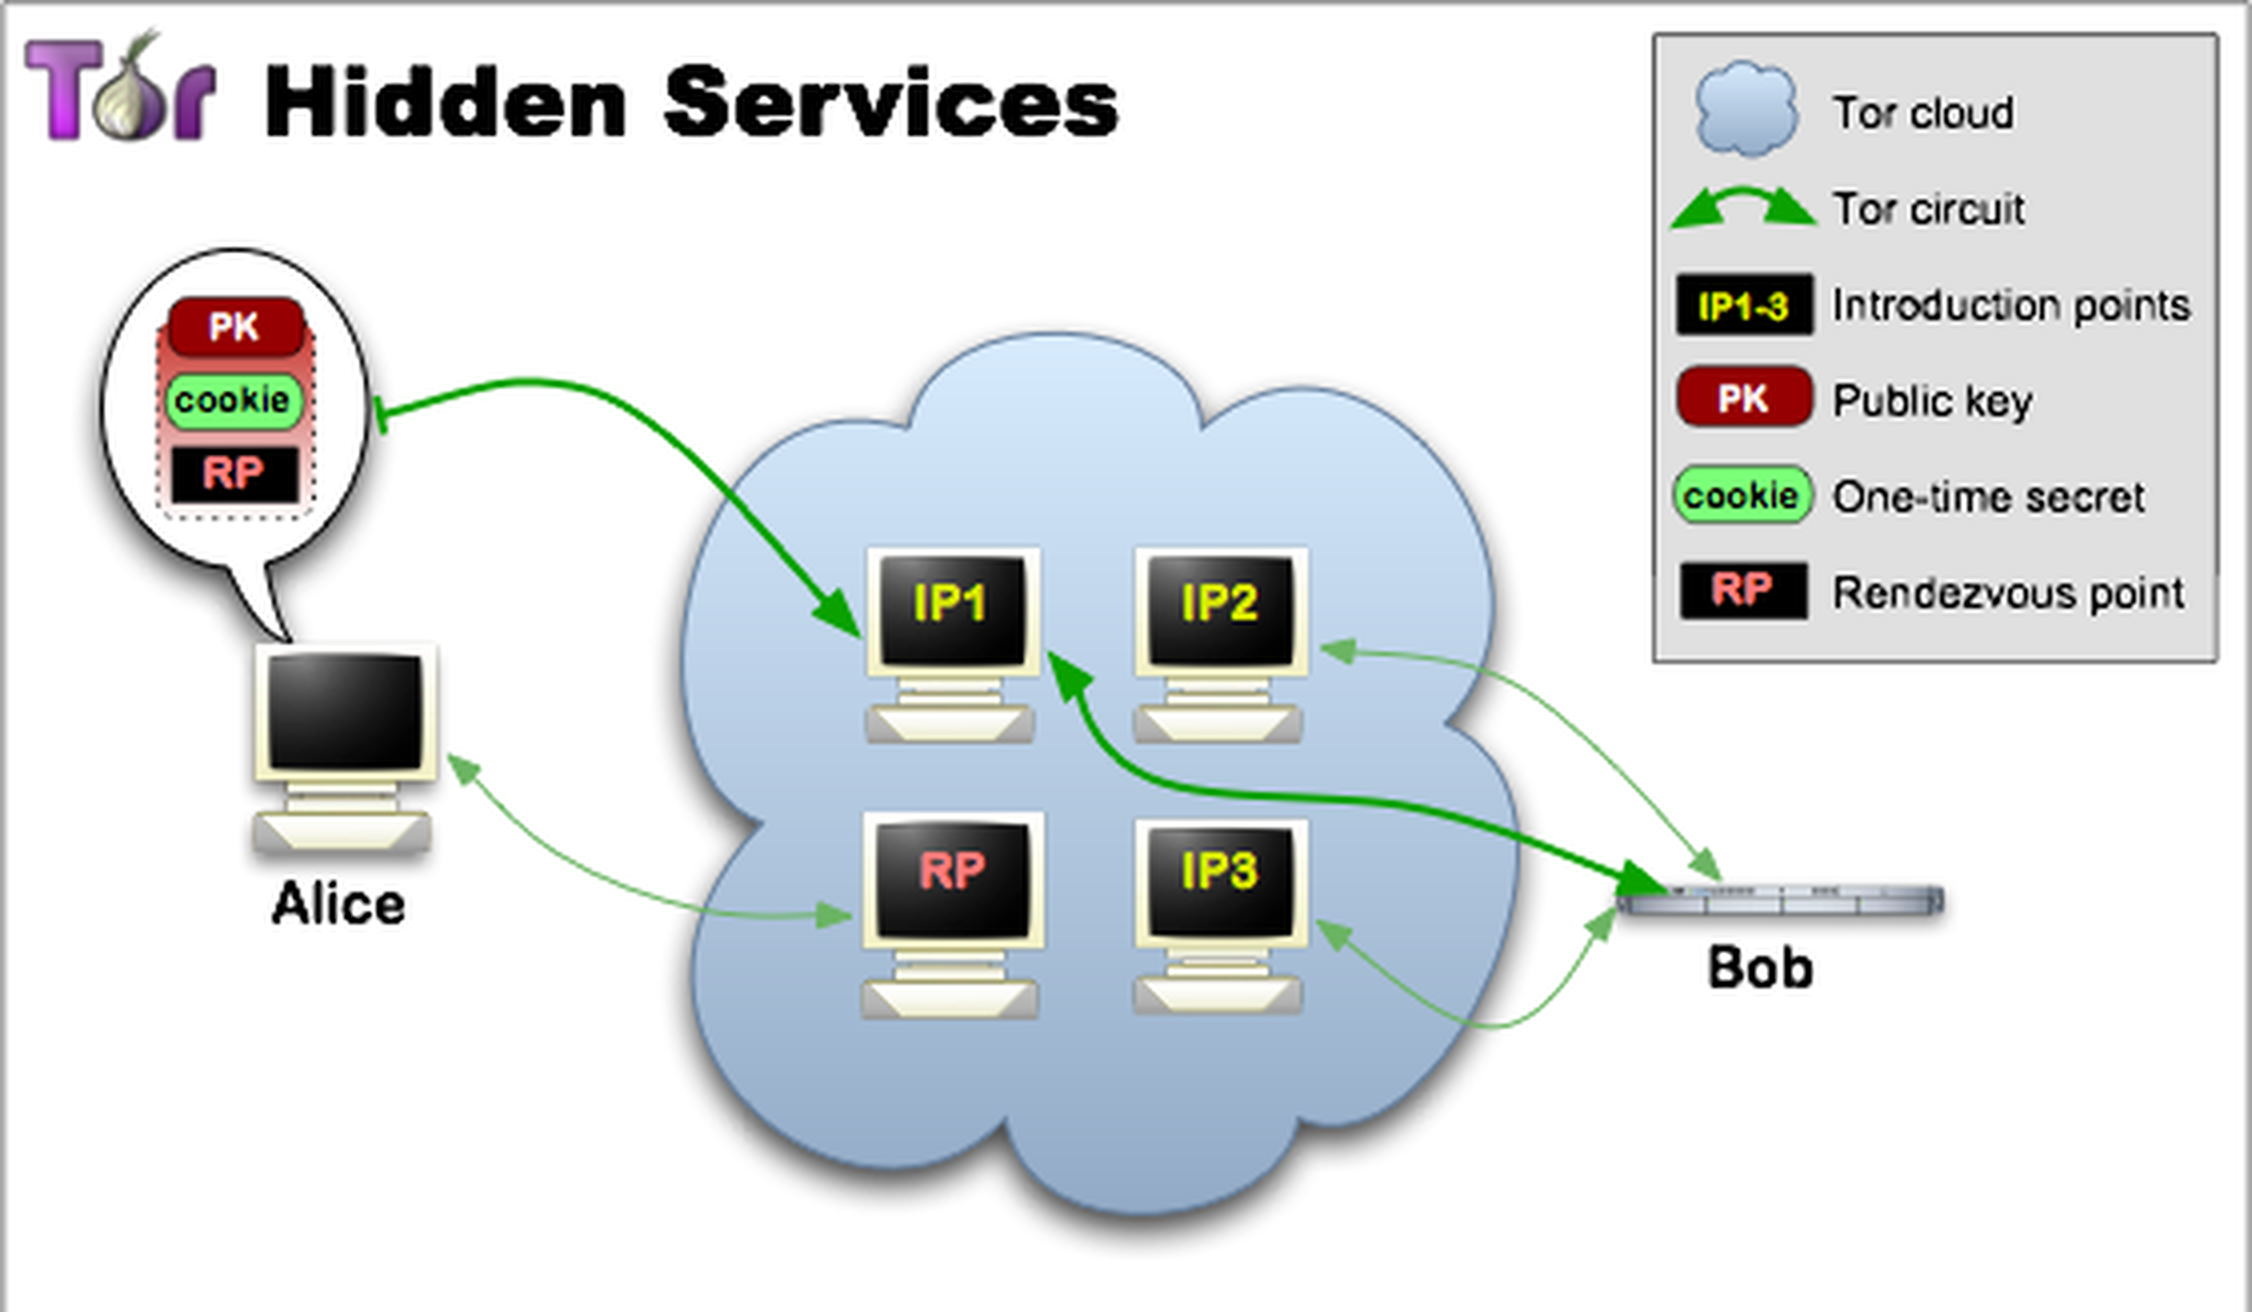
\includegraphics[width=\textwidth]{images/Tor/tor-hidden-service-4-higher.png}
%		\caption{Alice uses the encrypted cookie to tell Bob to switch to $ rp $.}
%	\end{minipage}
%	\hspace{0.5cm}
%	\begin{minipage}[b]{0.45\linewidth}
%		\centering
%		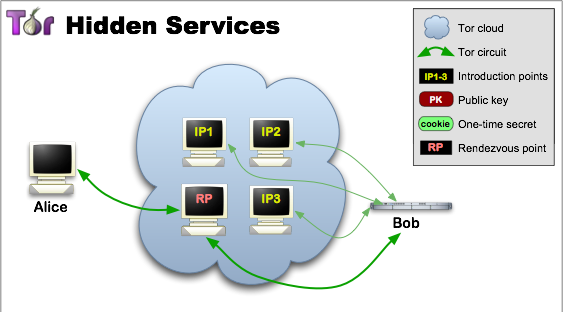
\includegraphics[width=\textwidth]{images/Tor/tor-hidden-service-6.png}
%		\caption{Bidirectional communication between Alice and the hidden service.}
%	\end{minipage}
%\end{figure}

She then sends to $ ip_{1} $ a cookie encrypted with $ B_{K} $, containing $ rp $ and $ sec $. Bob decrypts this message, builds a circuit to $ rp $, and tells it $ sec $, enabling Alice and Bob to communicate. Their communication travels through six Tor nodes: three established by Alice and three by Bob, so both parties remain anonymous. From there traditional HTTP, FTP, SSH, or other protocols can be multiplexed over this new channel.

As of March 2015, Tor hosts approximately 25,000 unique hidden services that together generate around 450 Mbit/s of traffic.\cite{TorMetrics}

\section{Motivation}
\label{sec:Motivation}

As Tor's hidden service addresses are algorithmically derived from the service's public RSA key, there is at best limited capacity to select a human-meaningful name. Some hidden service operators have attempted to work around this issue by finding an RSA key by brute-force that generates a partially-desirable hidden service address (e.g. ``example0uyw6wgve.onion'') and although some alternative encoding schemes have been proposed, (section \label{sec:EncodingSchemes}) the problem generally remains. The usability of hidden services is severely challenged by their non-intuitive and unmemorable base58-encoded domain name. For example, 3g2upl4pq6kufc4m.onion is the address for the DuckDuckGo search engine, \\ suw74isz7wqzpmgu.onion is a WikiLeaks mirror, and 33y6fjyhs3phzfjj.onion and \\ vbmwh445kf3fs2v4.onion are both SecureDrop instances for anonymous document submission. These addresses maintain strong privacy as the strong association between its public key and its address significantly breaks the association between the service's purpose and its address. However, this privacy comes at a cost: it is impossible to classify or label a hidden service's purpose in advance, a fact well known within Tor hidden service communities. Over time, third-party directories -- both on the Clear and Dark Internets -- appeared in attempt to counteract this issue, but these directories must be constantly maintained and furthermore this approach is not convenient nor does it scale well. This suggests the strong need for a more complete and reliable solution.

\section{Contributions}

Our contribution to this problem is six-fold:

\begin{itemize}
	\item We introduce a novel distributed naming system that enables Tor hidden service operators to choose a unique human-meaningful domain name and construct a strong association between that domain name and their hidden service address, squaring Zooko's Triangle (section \ref{sec:ZookosTriangle}).
	\item We described a new distributed, publicly confirmable, and partially self-healing transactional database.
	\item We provide OnioNS as a Tor plugin and rely on the existing Tor network and other infrastructure, rather than introduce a new network. This simplifies our assumptions and reduces our threat model to attack vectors already known and well-understood on the Tor network.
	\item We introduce a novel protocol for proving the non-existence of any domain name.
	\item We enable Tor clients to verify the authenticity of a domain name against its corresponding hidden service address with minimal data transfers and without requiring any additional queries.
	\item We preserve the privacy of both the hidden service and the anonymity of Tor clients connecting to it.
\end{itemize}

	
\chapter{PROBLEM STATEMENT}

\section{Assumptions and Threat Model}
\label{sec:Assumptions}

The design of OnionNS on several main assumptions and threat vectors:

\begin{itemize}
  \item Not all Tor nodes can be trusted. It is already well-known in the Tor community that some Tor nodes are run by malicious operators, curious researchers, experimenting developers, or government organizations. Nodes can be wiretapped, become semi-honest, or behave in an abnormal fashion. However, the majority of Tor nodes are honest and trustworthy: a reasonable assumption considering that Tor's large userbase must make this assumption when using Tor for anonymity or privacy-enhancement purposes.
  \item Let us define an ``honest node'' to mean that the node does not log data, is stable, kept up-to-date, and acts according to specifications. Let ``semi-honest'' mean that the node acts properly but may be logging data and ``dishonest'' to mean that the node is run by an attacker, logs data, and may behave improperly. For an $ M $-sized set chosen randomly from Tor nodes that have the stable and fast flags, $ \ceil[\big]{\frac{M}{2}} $ or more of them are at least semi-honest. This assumption is very similar to the assumption made when Tor clients create circuits: that all three nodes in a circuit are honest and less than all of them are semi-honest. Relays with stable and fast flags are have more consensus weight are thus more likely to be chosen relative to other nodes during circuit construction.
  \item The amount of dishonest Tor nodes does not increase in response to the inclusion of OnionNS into Tor infrastructure. Specifically, that if an attacker Eve can predict the next set of \emph{quorum} nodes (section \ref{sec:Quorum}) that Eve does not have enough time to make those nodes dishonest. This is a reasonable assumption because regular Tor traffic is far more valuable to an attacker than DNS data is, so penetration of the Tor network would have occurred already if Eve meant to introduce disruption. OnionNS data structures are almost all public anyway.
  \item Adversaries have access to some of Tor inter-node traffic and to portions of general Internet communication. However, attackers do not have not have a global view of Internet traffic; namely they cannot always correlate connections into the Tor network with connections out of the Tor network. This assumption is also made by the Tor community and developers. No attempt is made to defend against a global attacker from either Tor or OnionNS.
  \item Adversaries are not breaking properly-implemented Tor circuits and their modern components, namely TLS 1.2, the AES cipher, ECDHE key exchange, and the SHA2 series of digests, and that they maintain no backdoors in the Botan and OpenSSL implementations of these algorithms.
\end{itemize}

\section{Design Objectives}

Tor's high security environment is challenging to the inclusion of additional capabilities, even to systems that are backwards compatible to existing infrastructure. Anonymity, privacy, and general security are of paramount importance. We enumerate a short list of requirements for any secure DNS system designed for safe use by Tor clients. We later show how existing works do not meet these requirements and how we overcome these challenges with OnionNS.

\begin{enumerate}
	\item The registrations must be anonymous; it should be infeasible to identify the registrant from the registration.
	\item Lookups must be anonymous or at least privacy-enhanced; it should not be trivial to determine both a client's identity and the hidden service that the client is requesting.
	\item Registrations must be publicly confirmable; all parties must be able to verify that the registration came from the desired hidden service and that the registration is not a forgery. % todo: OnionNS should show the resolved .onion to confirm this
	\item Registrations must be securely unique, or have an extremely high chance of being securely unique such as when this property relies on the collision-free property of cryptographic hash functions.
	\item It must be distributed. The Tor community will adamantly reject any centralized solution for Tor hidden services for security reasons, as centralized control makes correlations easy, violating our first two requirements.
	\item It must remain simple to use. Usability is key as most Tor users are not security experts. Tor hides non-essential details like routing information behind the scenes, so additional software should follow suite. % suite, is that correct?
	\item It must remain backwards compatible; the existing Tor infrastructure must still remain functional.
	\item It should not be feasible to maliciously modify or falsify registrations in the database or in transit though insider attacks.
\end{enumerate}

Several additional objectives, although they are not requirements, revolve around performance: it should be assumed that it is impractical for clients to download the entirety or large portions of the DNS database in order to verify any of the requirements, a DNS system should take a reasonable amount of time to resolve domain name queries, and that the system should not introduce any significant load on client computers.

	
\chapter{\uppercase{Challenges}}

\section{Zooko's Triangle}

One of the largest challenges is inherent to the difficulty of designing a distributed system that maintains a correlation database of human-meaningful names in a one-to-one fashion. The problem is summarized in Zooko's Triangle, an influential conjecture proposed by Zooko Wilcox-O'Hearn in late 2001. The conjecture states that in a persistent naming system, only two out of the three following properties can be established:\cite{Ferdous2009}

\begin{itemize}
  \item Human meaningfulness: the names have a quality of meaningfulness and memorability to the users. 
  \item Securely unique: for any name, duplicates do not exist.
  \item Distributed: the naming system lacks a central authority or database for allocating and distributing names.
\end{itemize}

\begin{figure}[htbp]
	\centering
	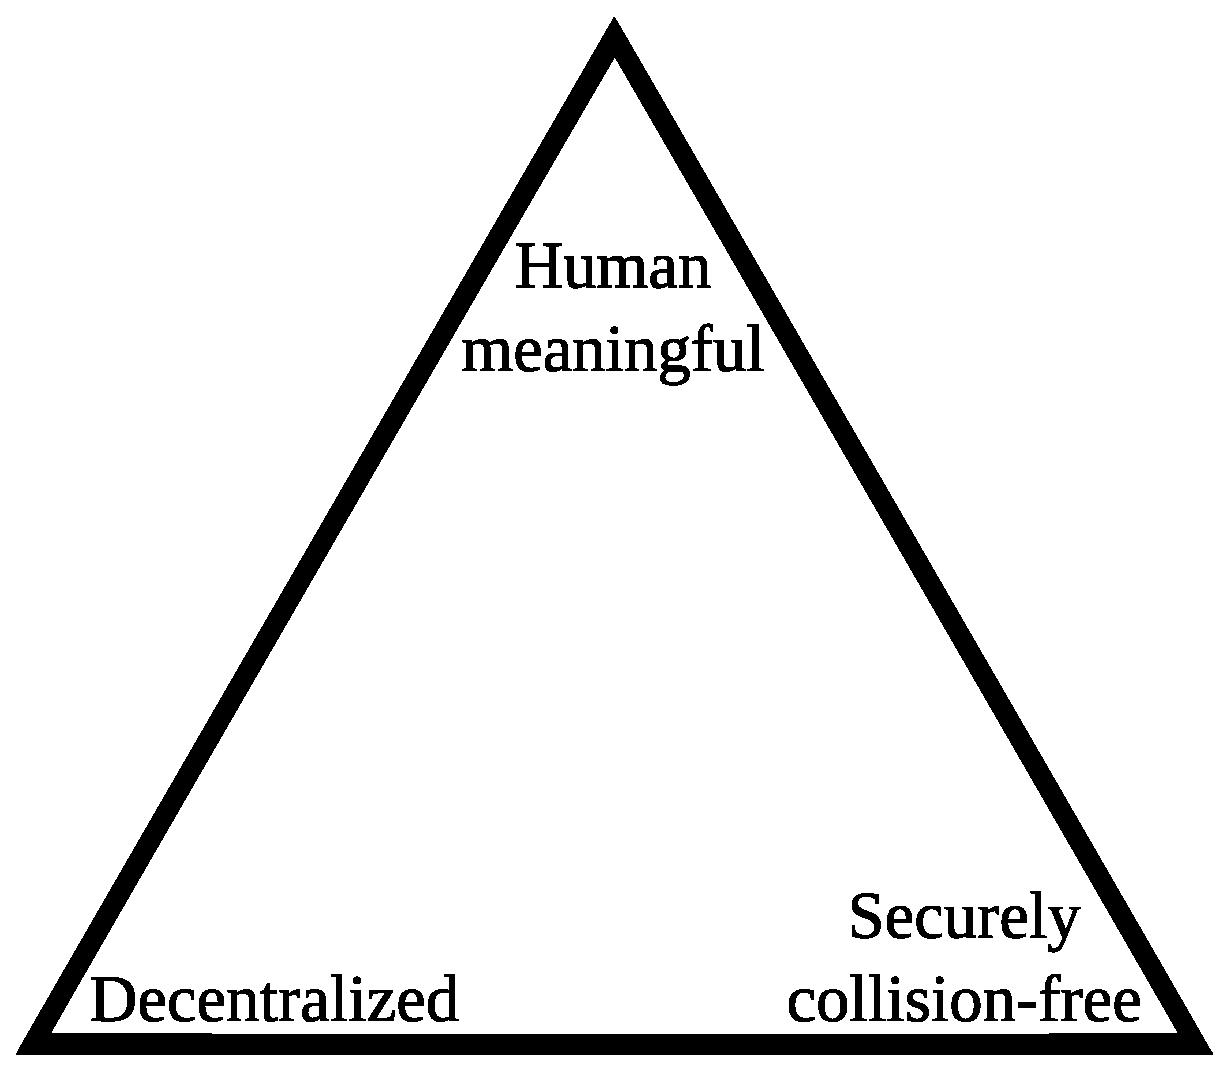
\includegraphics[width=0.3\textwidth]{images/Zooko.eps}
	\caption{Zooko's Triangle.}
	\label{fig:figure8}
\end{figure}

Tor hidden service .onion domains, PGP keys, and Bitcoin addresses are secure and decentralized but are not human-meaningful; they use the large key-space and the collision-free properties of secure digest algorithms to ensure uniqueness, so no centralized database is needed to provide this property. Tradition domain names on the Clearnet are memorable and provably collision-free, but use a hierarchical structure and central authorities under the jurisdiction of ICANN. Finally, human names and nicknames are meaningful and distributed, but not securely collision-free.\cite{Stiegler2005}

\section{Communication}



\section{Fault Tolerance}
	

\chapter{\uppercase{Existing Works}}

Existing literature proposing DNS systems for Tor is fairly sparse, though some ideas have been put forward.

\section{Clearnet DNS}

The Internet Domain Name Service (DNS) is a hierarchical distributed naming system for computers connected to the Internet. It links two principal Internet namespaces, Internet Protocol (IP) addresses and domain names, and translates one to the other. IP addresses specify the location of a computer or device on a network and domain names identify that resource. Domain names also serve as an abstraction layer so that devices can be moved to a different physical location or to a different IP address without loss of functionality. In contrast to IP addresses, domain names are human-meaningful and easily memorized, so DNS is a crucial component to the usability of the Internet.

Domain names on the Internet consist of a sequence of labels, delimited by dotes. The right-most label is the top-level domain (TLD) and can be used to classify the Internet resource by country or by organization type, although generic TLDs are more common. One or more subdomains follow the TLD. Each label can consist of up to 63 characters and the domain names can be up to 253 characters.



\section{Namecoin}

% TODO: expand: I spend six pages on Tor + hidden services, I should spend six pages on BTC + Namecoin, and two on DNS
% question: I'm aiming for 50 pages, and it looks I'll be burning 14 or 15 on introductions. Is that all right? If not, reduce to 5 + 5 + 1

Bitcoin is a decentralized peer-to-peer digital cryptocurrency, created by pseudonymous developer Satoshi Nakamoto in 2008. Ownership of Bitcoins consists of holding a private ECDSA key, and a transfer is a transmission of Bitcoins from one key to another. All transactions are recorded on a public ledger, called a blockchain, a data structure whose integrity is ensured through computational power but publically verifiable. Bitcoins are generated computationally at a fixed rate by \textit{miners} in a process that also secures the blockchain. Although Bitcoin received limited attention in the first two years of its life, it has since grown significantly since then, with approximately 70,000 daily transactions as of the time of this writing. Bitcoin's growth has led to the creation of many alternative cryptocurrencies, and its popularity has influenced financial discussions and legal controversy worldwide.

\subsection{Architecture}

A blockchain is data structure fundamental to Bitcoin, and crucial for its functionality. As a distributed decentralized system, this public ledger is Nakamoto's answer to the problem of ensuring agreement of critical data across all involved parties. The blockchain is a novel structure, and its structure guarantees integrity, chronological ordering of transactions, and the prevention of double-spending of Bitcoins. The blockchain consists of blocks of data that are held together by proof-of-work, a cryptographic puzzle whose solution is provably hard to find but trivial to verify. Bitcoin's proof-of-work is based on Adam Back's Hashcash scheme: that is, find a nonce such that the hash of this nonce and some data produces a result that begins with a certain number of zero bits. In Bitcoin's case this is stated as finding a nonce that when passed through two rounds of SHA256 ($ \textrm{SHA}256^{{2}} $) produces a value less than or equal to a target $ T $. This requires a party to perform on average $ \frac{1}{Pr[H \leq T]} = \frac{2 ^ {{256}}}{T} $ amount of computations, but it is easy to verify that $ \textrm{SHA}256^{{2}}(\textrm{msg} || n) \leq T $. Nodes in the Bitcoin network collectively agree to use the blockchain with the highest accumulation of computational effort, so an adversary seeking to modify the structure would need to recompute the proof-of-work for all previous blocks as well as out-perform the network, which is currently considered infeasible.\cite{Okupski2014}

Each block in the blockchain consists of a header and a payload. The header contains a hash of the previous block's header, the root hash of the Merkle tree built from the transactions in this block, a timestamp, a target $ T $, and a nonce. The block payload consists of a list of transactions. The root node of the Merkle tree ensures the integrity of the transaction vector: verifying that a given transaction is contained in the tree takes $ log(n) $ hashes, and a Merkle tree can be built $ n * log(n) $ time, ensuring that all transactions are accounted for. The hash of the previous block in the header ensures that blocks are ordered chronologically, and the Merkle root hash ensures that the transactions contained in each block are order chronologically as well. The target $ T $ changes every 2016 blocks in response to the speed at which the proof-of-work is solved such that Bitcoin miners take two weeks to generate 2016 blocks, or one block every 10 minutes. The $ \textrm{SHA}256^{{2}} $ proof-of-work provides integrity of the data structure, and secp256k1 ECDSA key are used to prove ownership of coins.\cite{Okupski2014}

\begin{figure}[htbp]
	\centering
	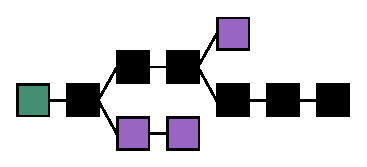
\includegraphics[width=0.6\textwidth]{images/Blockchain-2.eps}
	\caption{A sample blockchain.}
	\label{fig:figure6}
\end{figure}

\begin{figure}[htbp]
	\centering
	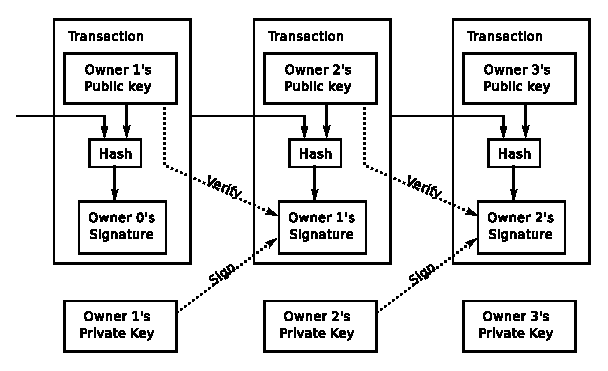
\includegraphics[width=0.6\textwidth]{images/bitcoin_transaction.eps}
	\caption{Three traditional Bitcoin transactions.}
	\label{fig:figure7}
\end{figure}

In the possibility that multiple nodes solve the proof-of-work and generate a new block simultaneously, the block becomes orphaned, the transactions recycled, and the blockchain follows the longest path from the genesis node to the latest block. Each transaction contains the public of the recipient, the ECDSA digital signature of the transaction from the sender, and the hash of the originating transaction. In this way, the digital signatures and proof-of-work in the blockchain can be traced back to the origin and forwards indefinitely. %In practice transactions can contain multiple input and outputs.

In recent years, systems have been developed that have shown Zooko's Triangle to be false. One prominent example is Namecoin, a naming system which uses a Bitcoin-like blockchain to store name-value pairs. Human-meaningful names can be embedded in the blockchain, which is distributed by nature. The uniqueness of the names is ensured by the Namecoin network and can be verified with anyone holding the blockchain. However, Tor developers have been wary of using Namecoin to store domain names for Tor hidden services. It is also impractical to require all Tor clients to download the entire blockchain before being able to use a hidden service DNS system, and there are inherent security challenges involved with querying servers or the Namecoin network for a registration without being able to use a complete blockchain to verify it. Therefore, another solution is needed.

Namecoin is a decentralized information registration and transfer system based on Bitcoin. It was the first software fork of Bitcoin and was introduced in April 2011. It uses its own blockchain and can hold name-value pairs in the blockchain attached to coins. While Bitcoin is primarily focused on supporting a currency, Namecoin aims to be a general key-value store, capable of holding cryptographic keys, DNS registrations, or other arbitrary data. It is most commonly used as a secure and censorship-resistance replacement for clearnet DNS. In 2014, Namecoin was recognized by ICANN is the most well-known example of a PKI and DNS system with an emphasis of distributed control and privacy, a growing trend in light of the revelations about the US Government by Edward Snowden. %https://www.icann.org/en/system/files/files/report-21feb14-en.pdf

\subsection{Names}

Although it inheriting Bitcoin's existing infrastructure, Namecoin added several transaction types specifically for registering and processing names, along with two new rules: names in the blockchain expire after 36,000 blocks unless renewed by the owner and no two unexpired names can be identical. These rules are enforced in the blockchain by Namecoin nodes and anyone verifying the Namecoin blockchain. Registering a name consumes 0.01 Namecoin, names can also be transferred to other owners, and they are two types: DNS and personal. The DNS type uses a new Top Level Domain (TLD) not in use by ICANN: .bit, and is used for DNS registrations. The personal name can contain arbitary data, including user information such as cryptographic keys. Like Bitcoin, Namecoin's maximum block size is one megabyte and the difficulty is set such that blocks generate every 10 minutes. Thus names expire every 250 days. 





\section{Different Encoding}

One of the most prominent is a 2011 Bachelor's thesis which outlines representing a hidden service's domain name as a series of words, rather than a base58-encoded hash.\cite{NicolussiThesis2011} However, while this scheme would improved recognition and memorability of hidden services, the words would remain random, are not chosen in advance, and do not relate to the hidden service in any meaningful way. Therefore this solution is an improvement but is not a solution. The problem remains open.
	
\chapter{SOLUTION}
\label{chapter:Solution}

% breadth-first explanation, examples inside protocol, explain only in context of Tor

% relative vs against

\section{Overview}

We propose the Onion Name Service, or OnioNS, a system which uses enables transparent translation of .tor domain names to .onion addresses. The system has three main aspects: the generation of self-signed claims on domain names by hidden service operators, the processing of domain information within the OnioNS servers, and the receiving and authentication of domain names by a Tor client.

First, a hidden service operator, Bob, generates an association claim between a meaningful domain name and a .onion address. Without loss of generality, let this be example.tor $ \rightarrow $ example0uyw6wgve.onion. For security reasons we do not introduce a central repository and authority from which Bob can purchase domain names; however, domains are not trivially obtainable and Bob must expend effort to claim and maintain ownership of example.tor. We achieve this through a proof-of-work scheme. Proof-of-work systems are noteworthy for their asymmetry: they require the issuer to spend effort to find an answer to a moderately hard computational problem, but once solved can be easily verified correct by any recipient. The requirement of proof-of-work fulfils three main purposes:

\begin{enumerate}
	\item Significantly reduces the threat of record flooding.
	\item Introduces a barrier-of-entry that encourages the utilization of domain names and the availability of the underlying hidden services.
	\item Increases the difficulty of domain squatting, a denial-of-service attack where a third-party claims one or more valuable domain names for the purpose of denying or selling them en masse to others. In Tor's anonymous environment, this vector is particularly prone to Sybil attacks.
\end{enumerate}

Bob then digitally signs his association and the proof-of-work with his service's private key.

Second, Bob uses a Tor circuit to anonymously transmit his association, proof-of-work, digital signature, and public key to OnioNS nodes, a subset of Tor routers. This set is deterministically derived from the volatile Tor consensus documents and is rotated periodically. The OnioNS nodes receive Bob's information, distribute it amongst themselves, and later archive it in a sequential transaction database, of which each OnioNS node holds their own copy. The nodes also digitally sign this database and distribute their signatures to the other nodes. Thus the OnioNS Tor nodes maintain a common database and have each vouched for its authenticity.

Third, a Tor client, Alice, uses a Tor client to anonymously connect to one of these OnioNS nodes and request a domain name. Without loss of generality, let this request be example.tor. Alice receives Bob's ``example.tor $ \rightarrow $ example0uyw6wgve.onion'' association, his proof-of-work, his digital signature, and his public key. Alice then verifies the proof-of-work and Bob's signature against his public key, and hashes his key to confirm the accuracy of example0uyw6wgve.onion. Alice then looks up example0uyw6wgve.onion in Tor's distributed hashtable, finds Bob's introduction point, and confirms that its knowledge of Bob's public key matches the key she received from the OnioNS nodes. Finally, she finishes the Tor hidden service protocol and begins communication with Bob. In this way, Alice can contact Bob through his chosen domain name without resorting to use lower-level hidden service addresses. The uniqueness and authenticity of the Bob's domain name is maintained by the subset of Tor nodes.

%At a high level, OnionNS' master page-chain is maintained by a randomly-selected rotating set of high-capacity Tor nodes. Other Tor nodes may mirror the page-chain, distributing the load and responsibilities across the network. The system supports a variety of command and control operations including Create, Domain Query, Onion Query, Modify, Move, Renew, and Delete.

% node vs server

% capitalize nouns that are defined

\section{Definitions}

To discuss OnioNS precisely we must first define some central terms that we will use throughout the rest of this document. We detail their exact contents in section \ref{sec:DataStructures} and how they are used throughout sections \ref{sec:BasicDesign} and \ref{sec:Protocols}.

\begin{description}
	\item[domain name] \hfill \\
		A \emph{domain name} is a case-insensitive identification string claimed by a hidden service operator. The syntax of OnioNS domain names mirrors the Internet DNS; we use a sequence of name-delimiter pairs with the .tor Top Level Domain (TLD). The TLD is a name at depth one and is preceded by names at sequentially increasing depth. The term ``domain name'' refers to the identiciation string as a whole, while ``second-level domain'' refers to the central name that is immediately followed by the TLD, as illustrated in Figure \ref{fig:sampleDomain}. Domain names point to \emph{destinations} -- other domain names with either the .tor or .onion TLD.

		\begin{figure}[htbp]
			\centering
			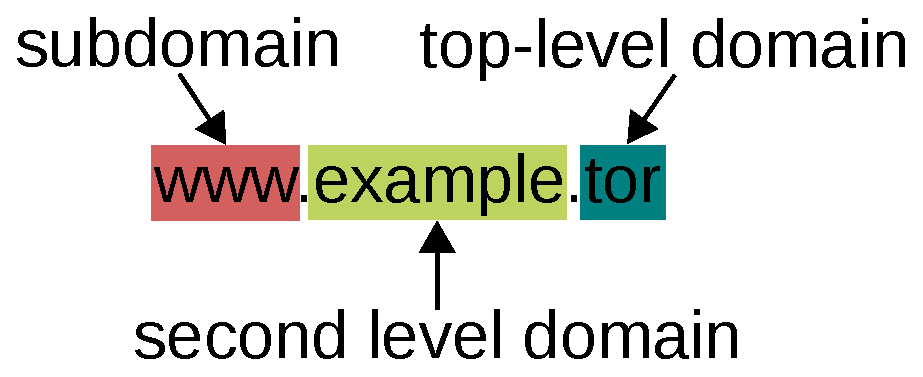
\includegraphics[width=0.5\textwidth]{images/domain-name.eps}
			\caption{A sample domain name: a sequence of labels separated by delimiters. In OnioNS, hidden service operators build associations between second-level domain names and their hidden service address.}
			\label{fig:sampleDomain}
		\end{figure}

	The Internet DNS defines a hierarchy of administrative realms that are closely tied to the depth of each name. By contrast, OnioNS makes no such distinction; we let hidden service operators claim second-level names and then control all names of greater depth under that second-level name. Hidden service operators may then choose to administer or sell the use of their subdomains, but this is outside the scope of this project.

	\item[Record] \hfill \\
		A \emph{Record} is a small textual data structure that contains one or more domain-destination pairs, a proof-of-work, a digital signature, and a public key. Records are issued by hidden service operators and sent to OnioNS servers. Every Record is self-signed with the hidden service's key. In section \ref{sec:Record} we describe the five different types of Records: Create, Modify, Move, Renew, and Delete. A Create Record represents a registration on an unclaimed second-level domain name, Modify, Move, and Renew are operations on that domain name or its subdomains, and a Delete Record relinquishes ownership over the second-level domain name and all its subdomains.

	\item[broadcast] \hfill \\
		The term for the protocol described in section \ref{sec:ProtoHiddenServices} that describes the uploading of new Records to OnioNS servers through Tor circuits and then the subsequent confirmation that the Record has been received.

	\item[Snapshot] \hfill \\
		A \emph{Snapshot} is textual database designed to hold collections of Records in a short-term volatile cache. They are also used to transmit sets of Records between OnioNS servers.

	\item[Page] \hfill \\
		A \emph{Page} is textual database designed to archive one or more Records in long-term storage. Pages are held and digitally signed by OnioNS nodes and are writable only for fixed periods of time before they are read-only. Each Page contains a link to a previous Page, forming an append-only public ledger known as an \emph{Pagechain}. This forms a two dimensional distributed data structure: the chain of Pages grows over time and there are multiple redundant copies of each Page spread out across the network at any given time.

	\item[Mirror] \hfill \\
		A \emph{Mirror} is any machine (inside or outside of the Tor network) that has performed a synchronization (section \ref{sec:Synchronization}) against the OnioNS network and now holds a complete copy of the Pagechain. Mirrors do not actively participate in the OnioNS network and do not have the power to manipulate the central page-chain.

	\item[Quorum Candidate] \hfill \\
		A \emph{Quorum Candidates} are \emph{Mirrors} inside the Tor network that have also fulfilled two additional requirements: 1) they must demonstrate that they are an up-to-date Mirror, and 2) that they have sufficient CPU and bandwidth capabilities to handle powering OnioNS in addition to their regular Tor duties. In other words, they are qualified and capable to power OnioNS, but have not yet been chosen to do so.

	\item[Quorum] \hfill \\
		A \emph{Quorum} is a subset of Quorum Candidates who have active responsibility over maintaining the master OnioNS Pagechain. Each Quorum node actively its own Page, which has a lifetime of that Quorum. The Quorum is randomly chosen from Quorum Candidates as described in section \ref{sec:ProtoTorClients}.

	\item[flood] \hfill \\
		The term for the periodic burst of communication that occurs between Quorum nodes wherein Snapshots are exchanged and each Quorum node obtains the state and digital signature of the current Page maintained by all other Quorum nodes. This communication is described in section \ref{sec:ProtoOnioNServers}.
\end{description}

\begin{figure}[htbp]
	\centering
	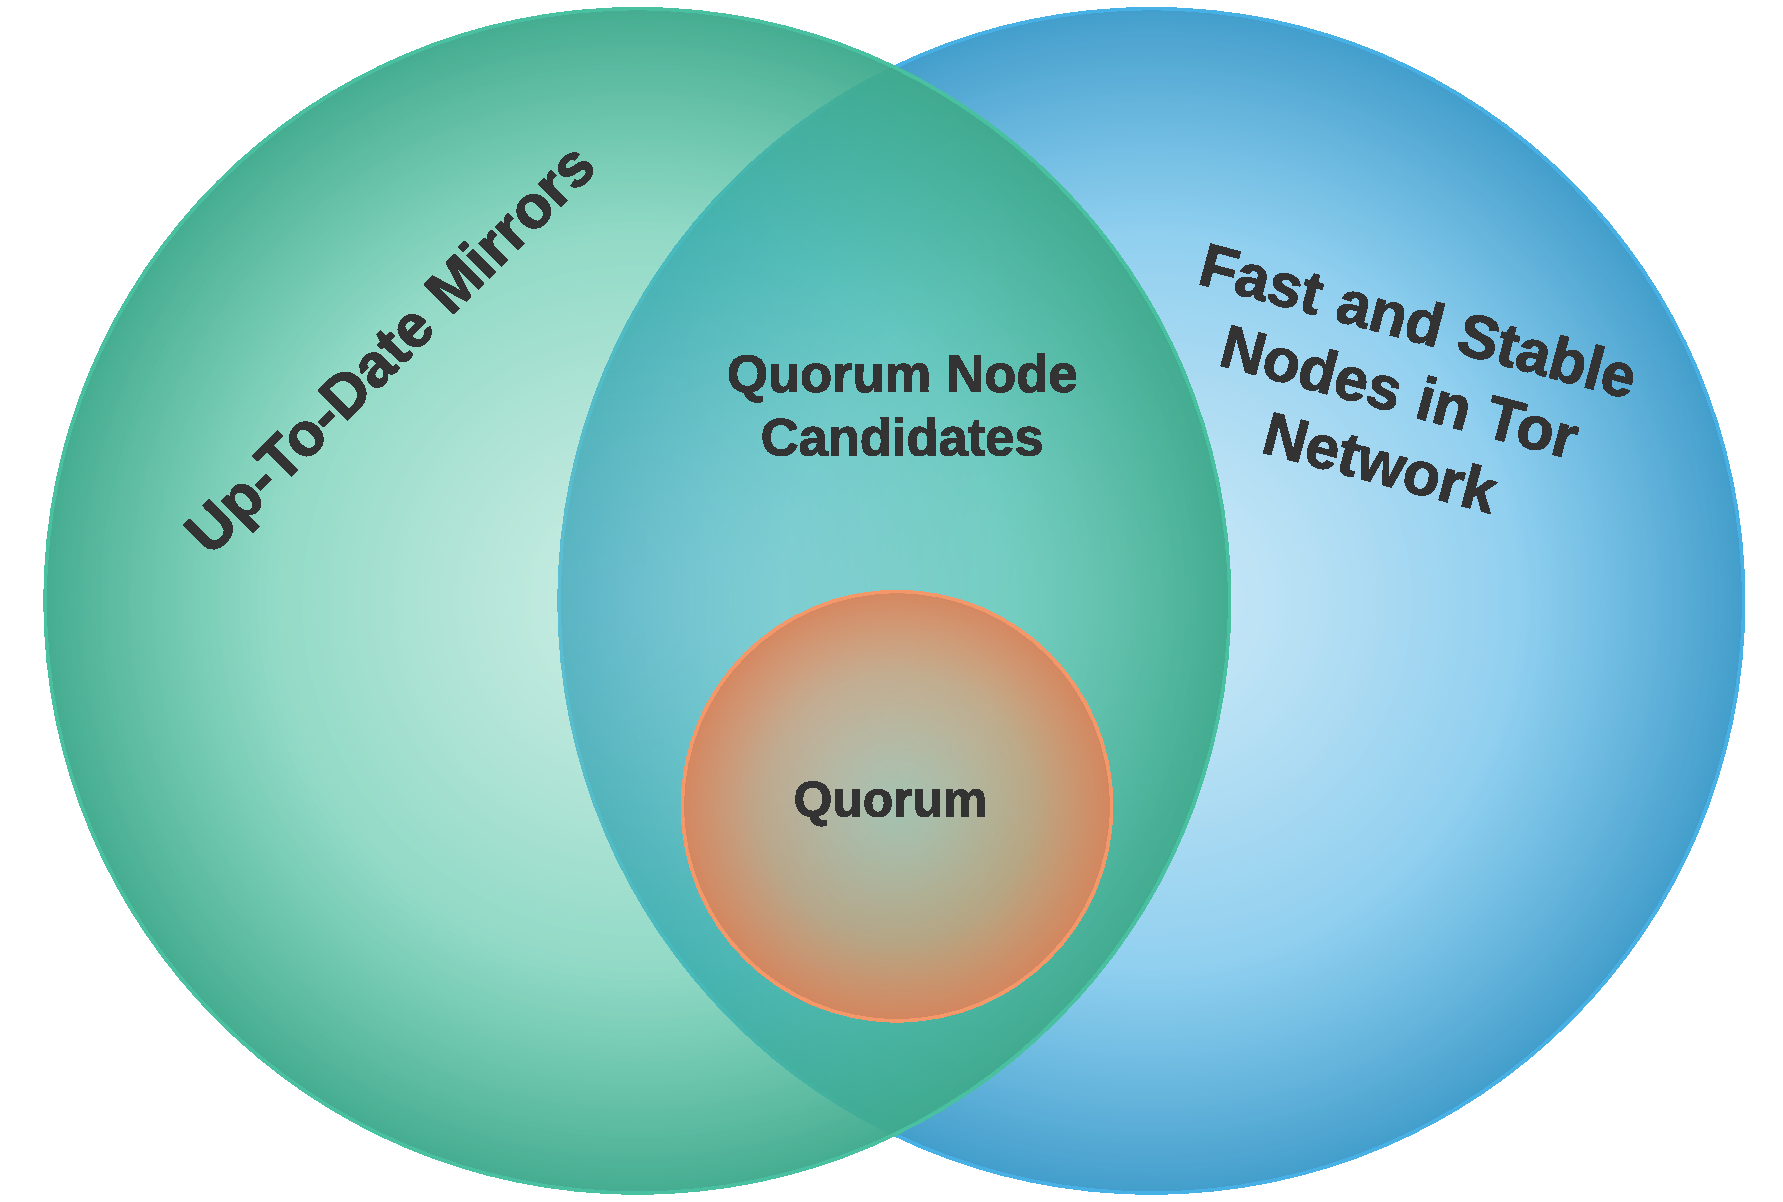
\includegraphics[width=0.5\textwidth]{images/LucidCharts/Participants.pdf}
	\caption{The relationship between Mirrors, Quorum Candidates, and the Quorum. A Mirror is any machine that holds the OnioNS Pagechain, Quorum Candidates are both up-to-date Mirrors and reliable Tor nodes, and the Quorum is randomly selected from the pool of Quorum Candidates.}
\end{figure}

Throughout the rest of this document, let Alice be a Tor client, and Bob be the operator of a hidden service. Assume that neither Alice nor Bob run Tor relays themselves, but let them only use Tor. Therefore Alice and Bob know the public keys of the Tor authority nodes and they can obtain and fully verify any past or current set of consensus documents. Bob has access to his hidden service private RSA key and may or may not have a PGP key with a subkey for email encryption.

\section{Basic Design}
\label{sec:BasicDesign}

OnioNS is build on a fundamental sequence of operations, as illustrated in Figure \ref{fig:basicDesign}:

\begin{enumerate}
	\item Bob generates a valid Record.
	\item Bob broadcasts the Record to the Quorum.
	\item The Record is flooded across the Quorum.
	\item Each Quorum node stores the Record into its current Page at the head of its local Pagechain.
	\item Alice queries the system for a domain name.
	\item Alice receives back the Record matching that domain name and confirms its validity.
	\item Alice connects to Bob via the hidden service protocol.
\end{enumerate}

These steps describe the propagation of any Record throughout the entire network. The protocols for each party are described in sections \ref{sec:ProtoHiddenServices}, \ref{sec:ProtoOnioNServers}, and \ref{sec:ProtoTorClients}, respectively. It should be noted that the activities of Alice, Bob, and the Quorum occur asynchronously: hidden service operator may be transmitting Records to the Quorum at the same time that clients are querying for other domain names.

\begin{figure}[htbp]
	\centering
	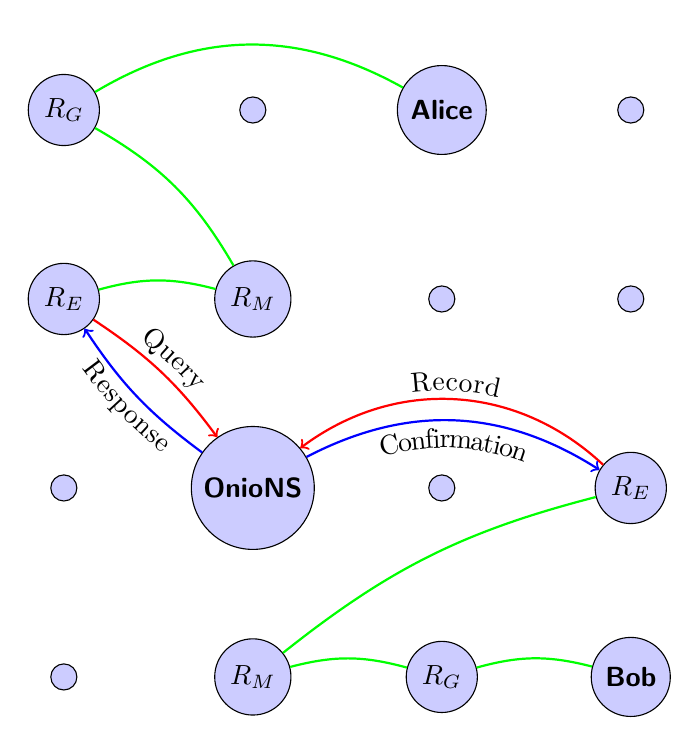
\begin{tikzpicture}[->, node distance=2.4cm, main node/.style={circle, fill=blue!20, draw, font=\sffamily\bfseries}]

			\node[main node] (1) {$ R_{G} $};
			\node[main node] (2) [right of=1] {};
			\node[main node] (3) [right of=2] {Alice};
			\node[main node] (4) [right of=3] {};

			\node[main node] (5) [below of=1] {$ R_{E} $};
			\node[main node] (6) [right of=5] {$ R_{M} $};
			\node[main node] (7) [right of=6] {};
			\node[main node] (8) [right of=7] {};

			\node[main node] (9) [below of=5] {};
			\node[main node] (10) [right of=9] {OnioNS};
			\node[main node] (11) [right of=10] {};
			\node[main node] (12) [right of=11] {$ R_{E} $};

			\node[main node] (13) [below of=9] {};
			\node[main node] (14) [right of=13] {$ R_{M} $};
			\node[main node] (15) [right of=14] {$ R_{G} $};
			\node[main node] (16) [right of=15] {Bob};

			% Alice-OnioNS conversation
			\tikzstyle{EdgeStyle}=[bend right, -, green]
			\Edge[](3)(1)
			\tikzstyle{EdgeStyle}=[bend left=15, -, green]
			\Edge[](1)(6)
			\Edge[](5)(6)
			\draw[thick, ->, red, postaction={decorate, decoration={text along path, text align=center, text={Query}, raise=4pt}}] (5) to [bend left=10] (10){};
			\draw[thick, <-, blue, postaction={decorate, decoration={text along path, text align=center, text={Response}, raise=-9pt}}] (5) to [bend right=10] (10){};

			% Bob-OnioNS conversation
			\tikzstyle{EdgeStyle}=[bend right=15, -, green]
			\Edge[](16)(15)
			\Edge[](15)(14)
			\tikzstyle{EdgeStyle}=[bend left=12, -, green]
			\Edge[](14)(12)
			\draw[thick, red, <-, postaction={decorate, decoration={text along path, text align=center, text={Record}, raise=3pt}}] (10) to [bend left=40] (12){};
			\draw[thick, blue, ->, postaction={decorate, decoration={text along path, text align=center, text={Confirmation}, raise=-10pt}}] (10) to [bend left=30] (12){};

		\end{tikzpicture}
	\caption{Bob uses a Tor circuit (guard, middle, and exit Tor routers) to anonymously broadcast a record to OnioNS. Alice uses her own Tor circuit to query the system for a domain name, and she is given Bob's record in response. Then Alice connects to Bob by Tor's hidden service protocol (section \ref{sec:HiddenServices}).}
	\label{fig:basicDesign}
\end{figure}

\subsection{Domain Name Operations}

Bob first generates a valid Record which he transmits over a Tor circuit to a randomly-selected Quorum node, who confirms acceptance or returns an error message otherwise. Bob's Record is flooded to the rest of Quorum via the periodic flushing of Snapshots by each Quorum node. Therefore, Bob can confirm that the rest of the Quorum received his Record by constructing another circuit to a different randomly-selected Quorum node and asking it for his Record. This process is illustrated in Figure \ref{fig:recordBroadcast}.

\begin{figure}[htbp]
	\centering
	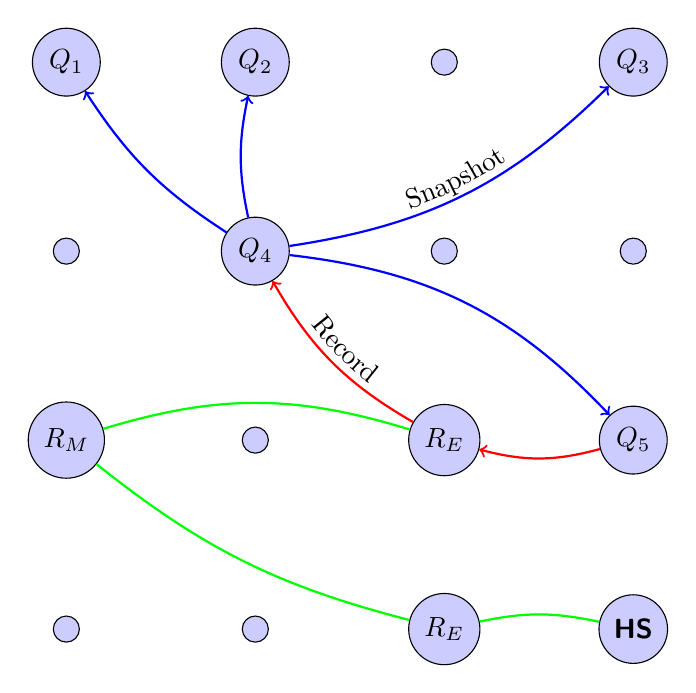
\begin{tikzpicture}[->, node distance=2.4cm, main node/.style={circle, fill=blue!20, draw, font=\sffamily\bfseries}]

			\node[main node] (1) {$ Q_{1} $};
			\node[main node] (2) [right of=1] {$ Q_{2} $};
			\node[main node] (3) [right of=2] {};
			\node[main node] (4) [right of=3] {$ Q_{3} $};

			\node[main node] (5) [below of=1] {};
			\node[main node] (6) [right of=5] {$ Q_{4} $};
			\node[main node] (7) [right of=6] {};
			\node[main node] (8) [right of=7] {};

			\node[main node] (9) [below of=5] {$ R_{M} $};
			\node[main node] (10) [right of=9] {};
			\node[main node] (11) [right of=10] {$ R_{E} $};
			\node[main node] (12) [right of=11] {$ Q_{5} $};

			\node[main node] (13) [below of=9] {};
			\node[main node] (14) [right of=13] {};
			\node[main node] (15) [right of=14] {$ R_{E} $};
			\node[main node] (16) [right of=15] {HS};

			% draw 1st and 2nd part of circuit
			\tikzstyle{EdgeStyle}=[bend right=12, -, green]
			\Edge[](16)(15)
			\Edge[](9)(15)

			% draw last part of circuit
			\tikzstyle{EdgeStyle}=[bend left=17, -, green]
			\Edge[](9)(11)

			% draw record moving from exit to 1st q. node
			\draw[thick, red, <-, postaction={decorate, decoration={text along path, text align=center, text={Record}, raise=3pt}}] (6) to [bend right=15] (11){};

			% draw verification with second q. node
			\draw[thick, red, ->, postaction={decorate}] (12) to [bend left=15] (11){};

			% draw upper left propegation
			\tikzstyle{EdgeStyle}=[bend left=12, ->, blue]
			\Edge[](6)(2)
			\Edge[](6)(1)

			% draw upper right propegation
			\tikzstyle{EdgeStyle}=[bend left=20, ->, blue]
			\Edge[](6)(12)
			\draw[thick, blue, postaction={decorate, decoration={text along path, text align=center, text={Snapshot}, raise=3pt}}] (6) to [bend right=18] (4){};

		\end{tikzpicture}
	\caption{Bob uses his existing circuit (green) to inform Quorum node $ Q_{4} $ of the new record. $ Q_{4} $ then floods it via Snapshots to all other Quorum nodes. Each node stores it in their own Page for long-term storage. Bob confirms from another Quorum node $ Q_{5} $ that his Record has been received.}
	\label{fig:recordBroadcast}
\end{figure}

\subsection{Pagechain Maintenance}

The Pagechain is OnioNS' fundamental data structure and is the central component of the entire system. It is a distributed append-only transactional database of a fixed maximum length. Each Page references a previous Page, forming a long chain. The head of the chain (the latest Page) is maintained and digitally signed by each member of the current Quorum. The Pagechain is designed as a public and fully confirmable data structure -- that is, any Mirror can check the integrity of each Page and the Records contained within them, the uniqueness of domain names, and the validity of the digital signatures on each Page from all Quorum nodes.

Any Mirror may continue its own Pagechain by generating a new Page, adding that Page to the front of its Pagechain, deleting the oldest Page, and then merging new Records into the new Pagechain head. When a Quorum Candidate is chosen as a Quorum node, it modifies its local Pagechain in this way. Assuming that the entire Quorum is honest and maintains perfect flooding communication, the entire Quorum would be in agreement. However, any Quorum node may experience downtime and may miss Snapshot broadcasts, have data corruption, act maliciously, or have other cause for its Pagechain head to deviate relative to the others. Therefore, disagreements may inevitably form within the Quorum. We address this under our original assumption that the largest set of Quorum nodes that have matching and valid Pagechains are also acting honestly. Therefore each Mirror can follow this rule to derive the master Pagechain and safely ignore any ``sidechains''. Likewise, each new honest Quorum member follows suite when creating a new Page, as described in section \ref{sec:ProtoOnioNServers}. Thus the Pagechain is at least partially self-healing. We illustrate this in Figure \ref{fig:sidechains}.

\begin{figure}[htbp]
	\centering
	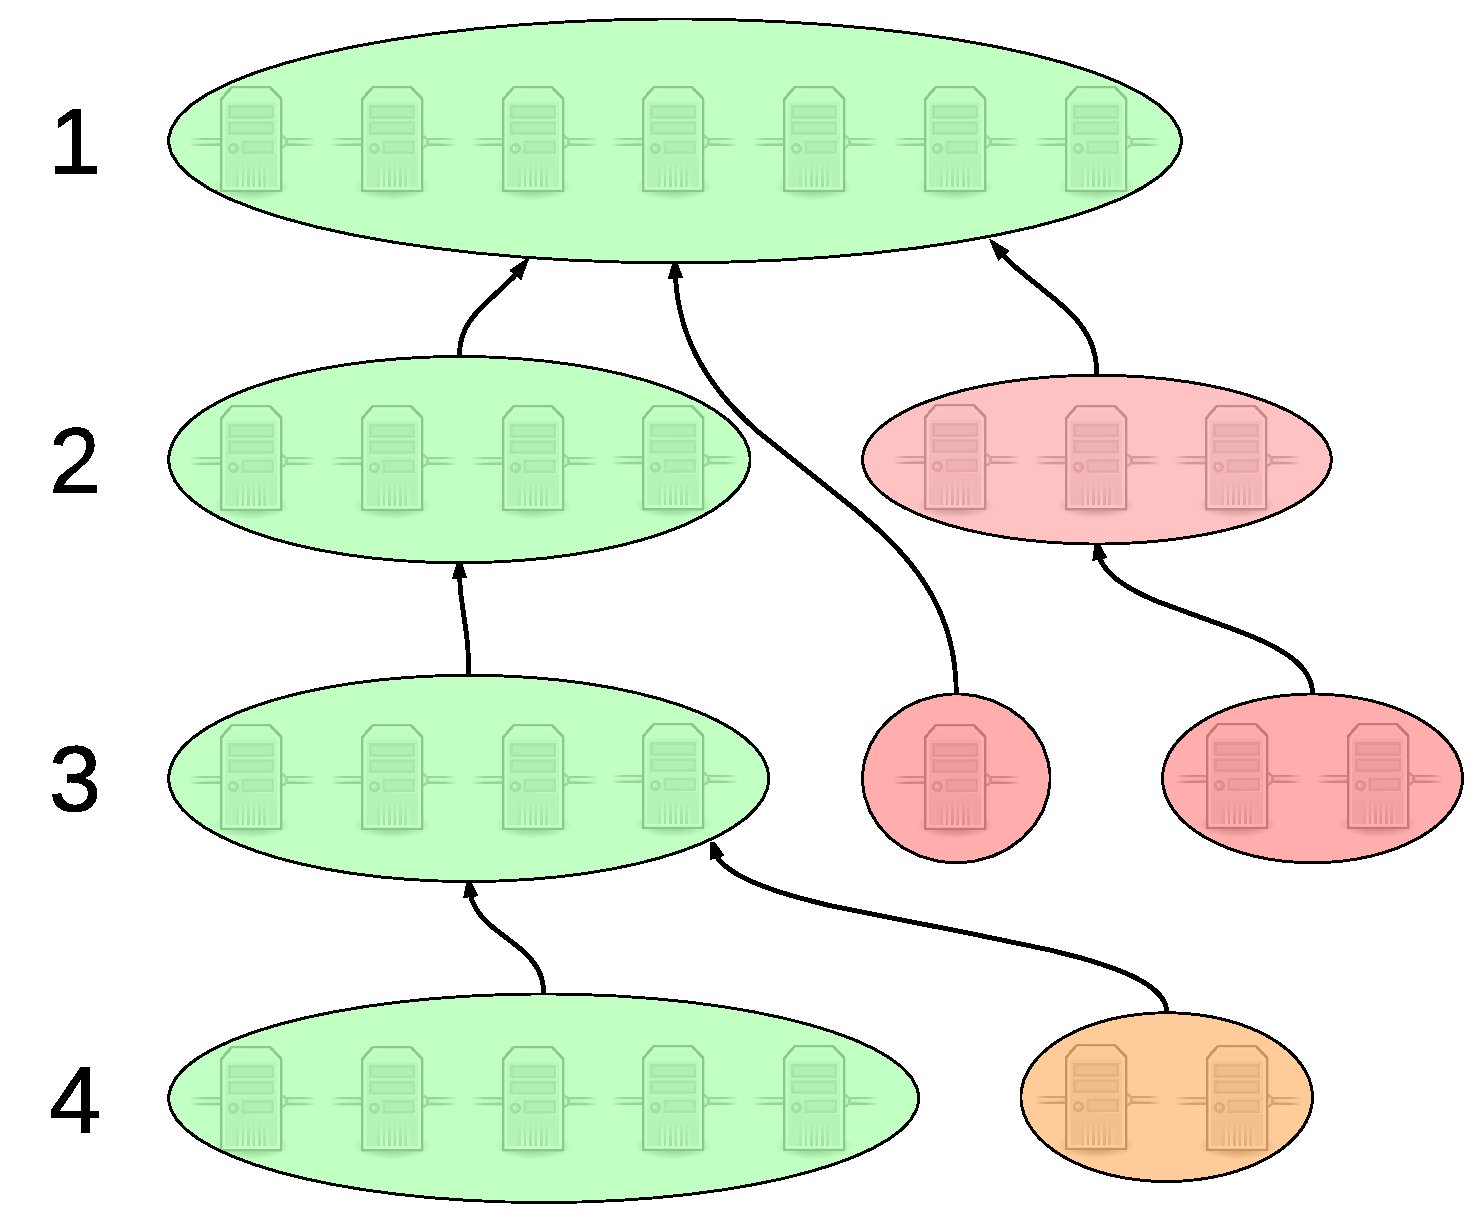
\includegraphics[width=0.65\textwidth]{images/LucidCharts/Page-chain.pdf}
	\caption{An example Pagechain across four Quorums. Each Page contains a references to a previous Page, forming a distributed append-only chain. $ \mathrm{Quorum}_{1} $ is honest and maintains reliable flooding communication, and thus has identical Pages. $ \mathrm{Quorum}_{2} $'s largest cluster is likewise in agreement, but there are three nodes which are acting maliciously together and have changed their Pages. Node 5 in $ \mathrm{Quorum}_{3} $ references an old page in attempt to bypass $ \mathrm{Quorum}_{2} $'s records, and nodes 6-7 are colluding with nodes 5-7 from $ \mathrm{Quorum}_{2} $. Finally, $ \mathrm{Quorum}_{4} $ has two nodes that acted honestly but did not record new records, so their Pagechains differ from the others. However, across all four days the largest clusters are honest nodes and thus integrity remains in the master Pagechain.}
	\label{fig:sidechains}
\end{figure}

\subsection{Client Request}
\label{sec:ClientRequest}

% todo: make diagram of this

Let Bob and Dave be two hidden services, and assume that OnioNS knows a Record from Bob containing an ``example.tor $ \rightarrow $ example0uyw6wgve.onion'' association, and a Record from Dave containing ``example2.tor $ \rightarrow $ example5chqt7to6.onion, sub.example2.tor $ \rightarrow $ example.tor''. Now let Alice request ``sub.example2.tor''.

Since the .tor TLD is not used by the Internet DNS, Alice's client software must direct the request through a Tor circuit to some OnioNS resolver, $ O_{r} $. By default, $ O_{r} $ belongs to the set of Quorum Candidate nodes although Alice may override this and choose some Mirror if she wishes. For security and load reasons, Quorum nodes refuse to respond to queries, so Alice cannot ask them. Following Alice's request, $ O_{r} $ searches its local Pagechain for ``example2.tor'' and finds Dave's Record, which it then sends to Alice. Alice sees the ``sub.example2.tor $ \rightarrow $ example.tor'' association and now queries $ O_{r} $ for ``example.tor''. $ O_{r} $ then locates and sends Bob's Record to Alice. Alice sees that ``example.tor'' has a destination of ``example0uyw6wgve.onion'', and because it has a .onion address she does not need to issue any more queries. Instead, Alice connects to Bob's example0uyw6wgve.onion service via the Tor hidden service protocol and sends her original request (``sub.example2.tor'') to Bob. As is the case with the Internet, Bob's web server may or may not provide specific content to Alice based on this request, but his configuration is outside our scope.

In this way, Alice can query an OnioNS resolver for some Dave-selected domain name and recursively resolve it to a .onion address transparently. The number of resolutions Alice makes is fixed to a maximal length (section \ref{sec:Record}) so this algorithm always completes. We discuss minor optimizations and security enhancements to this procedure in section \ref{sec:ProtoTorClients}.

\section{Primitives}

\subsection{Cryptographic}
\label{sec:CryptoPrim}

OnionNS makes use of cryptographic hash algorithms, digital signatures, proof-of-work, and a pseudorandom number generator.

\begin{itemize}
	\item Let $ H(x) $ be a cryptographic hash function. In our reference implementation we define $ H(x) $ as SHA-384, a truncated and slight modificated derivative of SHA-512. Currently the best preimage attack of SHA-512 breaks 57 out of 80 rounds in $ 2^{511} $ time.\cite{li2012converting} SHA-384 is included in the National Security Agency's Suite B Cryptography for protecting information classified up to Top Secret.
	\item Let $ S_{d}(m, r) $ be a deterministic RSA digital signature function that accepts a message $ m $ and a private RSA key $ r $ and returns an RSA digital signature. Let $ S_{d}(m, r) $ use $ H(x) $ as a digest function on $ m $ in all use cases. In our reference implementation we define $ S_{d}(m, r) $ as EMSA-PSS, (EMSA4) a probabilistic signature scheme defined by PKCS1 v2.1 and republished in 2003's RFC 3447.
	\item Let $ S_{\mathit{ed}}(m, c) $ be an Ed25519 digital signature function that accepts a message $ m $ and a private Curve25519 key $ c $ and returns a 64-byte Ed25519 digital signature. Ed25519 is digital signature scheme designed with high performance, strong implementation security, and minimal keypair and signature sizes objectives in mind. The Ed25519 elliptic curve is birationally equivalent to Curve25519, and Curve25519 keys can be converted to Ed25519 keys in $ \mathcal{O}(1) $ time.\cite{bernstein2011high} Let $ S_{\mathit{ed}}(m, c) $ use $ H(x) $ as a digest function on $ m $ in all use cases.
	\item Let $ V_{\mathit{ed}}(m, C) $ validate an Ed25519 digital signature by accepting a message $ m $ and a public Curve25519 key $ C $, and return true if the signature is valid. Let $ V_{\mathit{ed}}(m, C) $ use $ H(x) $ as a digest function on $ m $ in all use cases.
	\item Let $ \mathrm{PoW}(i) $ be a proof-of-work scheme such as a strong key derivation function that accepts an input key $ k $ and returns a derived key. Our reference implementation uses a fixed salt and scrypt, a password-based key derivation function which is notable for its large memory and CPU requirements during its operation. The scrypt function provides significantly greater resistance to custom hardware attacks and massively parallel computation primarily due to its memory requirements. This limits attackers to the same software implementation and asymptotic cost as legitimate users.\cite{percival2009stronger}\cite{percival2012scrypt} We choose scrypt because of these advantages over other key derivation functions such as SHA-256 or PBKDF2. For these reasons scrypt is also common for proof-of-work purposes in some cryptocurrencies such as Litecoin.
	\item Let $ \mathit{R}(s) $ be a pseudorandom number generator that accepts an initial seed $ s $ and returns a list of numerical pseudorandom numbers. We suggest MT19937, commonly known as the Mersenne Twister. This generator is widely used throughout most programming languages and is well known for its speed, long period, and the high quality of its pseudorandom output, although it is not cryptographically secure.\cite{matsumoto1998mersenne}
\end{itemize}

\subsection{Symbols}

\begin{itemize}
	\item Let $ L_{Q} $ represent size of the Quorum.
	\item Let $ L_{T} $ represent the number of routers in the Tor network.
	\item Let $ L_{P} $ represent the maximum number of Pages in the Pagechain.
	\item Let $ q $ be an Quorum iteration counter.
	\item Let $ \Delta q $ be the lifetime of a Quorum in days: every $ \Delta q $ days $ q $ is incremented by one and a new Quorum is chosen.
	\item Let $ s $ be a Snapshot iteration counter.
	\item Let $ \Delta s $ be the lifetime of a Snapshot in days: every $ \Delta s $ minutes $ s $ is incremented by one, a flood happens, and a fresh Snapshot is used.
\end{itemize}

All textual databases are encoded in JSON. JSON is significantly more compact than XML, but retains readability. Its support of basic primitive types is highly applicable to our needs. Additionally, we consider the JSON format safer than byte-level encoding.

\section{Data Structures}
\label{sec:DataStructures}

\subsection{Record}
\label{sec:Record}

There are five different types of Records: Create, Modify, Move, Renew, and Delete. The latter four Records mimic the format of the Create Record with minor exceptions.

\subsubsection{Create}

A Create record consists of nine components: \emph{type}, \emph{nameList}, \emph{contact}, \emph{timestamp}, \emph{consensusHash}, \emph{nonce}, \emph{pow}, \emph{recordSig}, and \emph{pubHSKey}. Fields that are optional are blank unless specified, and all fields are encoded in base64, except for \emph{nameList} and \emph{timestamp}, which are encoded in standard UTF-8.

\renewcommand{\arraystretch}{1.75} % increase spacing between columns
\begin{center}
    \begin{longtabu}{ | l | c | p{9.5cm} |}
    \hline
    \textbf{Field} & \textbf{Required?} & \textbf{Description} \\
    type & Yes & A textual label containing the type of Record. In this case, \emph{type} is set to ``Create''. \\
    nameList & Yes & An array list of domain names and their destinations. The list of domain names includes one or more second-level domain name, while the remainder of the list contains zero or more subdomains (names at level $ < 2 $) under that second-level domains. In this way, records can be referenced by their unique second-level domain names. Destinations use either .tor or .onion TLDs. \\
    contact & No & Bob's PGP key fingerprint, if he has a key and chooses to disclose it. If the fingerprint is listed, clients may query a public keyserver for this fingerprint, obtain the PGP public key, and contact Bob over encrypted email. \\
    timestamp & Yes & The UNIX timestamp of when the issuer created the registration and began $ \mathrm{PoW}(i) $. \\
    consensusHash & Yes & The hash of the consensus document that generated $ \mathit{Quorum}_{q} $ \\
    nonce & Yes & Four bytes that serve as a source of randomness for $ \mathrm{PoW}(i) $. \\
   	pow & Yes & 16 bytes that store the output of $ \mathrm{PoW}(i) $. \\
   	recordSig & Yes & The output of $ S_{d}(m, r) $ where $ m = \mathit{nameList} \concat \mathit{timestamp} \concat \mathit{consensusHash} \concat \mathit{nonce} \concat \mathit{pow} $ and $ r $ is the hidden service's private RSA key. \\
   	pubHSKey & Yes & Bob's public RSA key. \\
    \hline
    \caption{A Create record, which contains fields common to all records. Every record is self-signed and must have verifiable proof-of-work before it is considered valid.}
    \end{longtabu}
\end{center}

\subsubsection{Modify}

A Modify record allows an owner to update his registration with updated information. The Modify record has identical fields to Create, but \emph{type} is set to ``Modify''. The owner corrects the fields, updates \emph{timestamp} and \emph{consensusHash}, revalidates the proof-of-work, and transmits the record. Modify records have a difficulty of $ \frac{\textrm{difficulty}_{\textrm{Create}}}{4} $. Modify records can be used to add and remove domain names but cannot be used to claim additional second-level domains.

\subsubsection{Move}

% prevents the seller from selling modified records and forcing the buyer to issue a Modify record

A Move record is used to transfer one or more second-level domain names and all associated subdomains from one owner to another. Move records have all the fields of a Create record, have their \emph{type} is set to ``Move'', and contain two additional fields: \emph{target}, a list of domain-destination pairs, and \emph{destPubKey}, the public key of the new owner. Domain names and their destinations contained in \emph{target} cannot be modified; they must match the latest Create, Renew, or Modify record that defined them. Move records also have a difficulty of $ \frac{\textrm{difficulty}_{\textrm{Create}}}{4} $.

\subsubsection{Renew}

% put "page" in italics everywhere?

Second-level domain names (and their associated domain names) expire every $ L $ days because (as explained below) the page-chain has a maximum length of $ L $ pages. Renew records must be reissued periodically at least every $ L $ days to ensure continued ownership of domain names. Renew records are identical to Create records, except that \emph{type} is set to ``Renew''. No modifications to existing domain names can be made in Renew records, and the domain names contained within must already exist in the page-chain. Similar to the Modify and Move records, Renew records have a difficulty of $ \frac{\textrm{difficulty}_{\textrm{Create}}}{4} $.

\subsubsection{Delete}

% attacker could compromise key, issues Move record before original owner knew of compromise. Or attacker could then reclaim domain name

If a owner's private key is compromised or if they wish to relinquish ownership rights over all of their domain names, they can issue a Delete record. Aside from their \emph{type} field set to ``Delete'', Delete records are identical in form to Create records but have the opposite effect: all second-level domains contained within the record are purged from local caches and made available for others to claim. There is no difficulty associated with Delete records, so they can be issued instantly.

\subsection{Snapshot}

Snapshots contain four fields: \emph{originTime}, \emph{recentRecords}, \emph{fingerprint}, and \emph{snapshotSig}.

\begin{description}
	\item[originTime] \hfill \\
		Unix time when the snapshot was first created.
	\item[recentRecords] \hfill \\
		A array list of records in reverse chronological order by receive time.
	\item[fingerprint] \hfill \\
		The hash of the public key of the machine maintaining this snapshot. This is the Tor fingerprint, a unique identification string widely used throughout Tor infrastructure and third-party tools to refer to specific Tor nodes.
	\item[snapshotSig] \hfill \\
		The output of $ S_{\mathit{ed}}(\mathit{originTime} \concat \mathit{recentRecords} \concat \mathit{fingerprint}], c) $ where $ c $ is the machine's private Curve25519 NTor key.
\end{description}

\subsection{Page}

Each page contains five fields, \emph{prevHash}, \emph{recordList}, \emph{consensusDocHash}, \emph{fingerprint}, and \emph{pageSig}.

\begin{description}
	\item[prevHash] \hfill \\
		The SHA-384 hash of \emph{prevHash}, \emph{recordList}, and \emph{consensusDocHash} of a previous page.
	\item[recordList] \hfill \\
		An array list of records, sorted in a deterministic manner.
	\item[consensusDocHash] \hfill \\
		The SHA-384 of $ cd $.
	\item[fingerprint] \hfill \\
		The hash of the public key of the machine maintaining this page, the Tor fingerprint.
	\item[pageSig] \hfill \\
		The output of $ S_{\mathit{ed}}(H(\mathit{prevHash} \concat \mathit{recordList} \concat \mathit{consensusDocHash})], c) $ where $ c $ is the machine's private Curve25519 NTor key.
\end{description}

\section{Protocols}
\label{sec:Protocols}

Throughout this section, when a party downloads consensus documents, they can safely obtain them from any source because they can validate the signatures on the documents against the Tor authority public keys to ensure that they were not modified in transit. Several online sources archive consensus documents and make them available retrospectively; in our reference implementation we also introduce another source. Note that in practice it is often more efficient to download consensus documents en-masse as they achieve very high compression ratios under 7zip.

% todo: the examples here aren't valid

\subsection{Hidden Services}
\label{sec:ProtoHiddenServices}

\subsubsection{Record Generation}

Mirrors and Tor clients check the validity of Records that they receive through synchronization or query responses, respectively. Invalid Records will be rejected by all parties, so Bob must generate a valid Record before broadcast.

\begin{enumerate}
	\item Bob selects the value for \emph{type} based on the desired operation.
	\item Bob constructs the \emph{nameList} domain-destination associations.
	\item Bob provides his PGP key fingerprint in \emph{contact} or leaves it blank if he doesn't have a PGP key or if he chooses not to disclose it. Bob can derive his PGP fingerprint with the ``gpg --fingerprint'' Unix command.
	\item Bob records the number of seconds since the Unix epoch in \emph{timestamp}.
	\item Bob sets \emph{consensusHash} to the output of $ H(x) $, where $ x $ is the consensus document published at 00:00 GMT on day $ \floor[\big]{\frac{q}{\Delta q}} $.
	\item Bob initially defines \emph{nonce} as four zeros.
	\item Let $ \mathit{central} $ be $\mathit{type} \concat \mathit{nameList} \concat \mathit{contact} \concat \mathit{timestamp} \concat \mathit{consensusHash} \concat \mathit{nonce} $.
	\item Bob sets \emph{pow} as $ \mathrm{PoW}(\mathit{central}) $.
	\item Bob sets \emph{recordSig} as the output of $ S_{d}(m, r) $ where $ m = \mathit{central} \concat \mathit{pow} $ and $ r $ is Bob's private RSA key.
	\item Bob saves the PKCS.1 DER encoding of his RSA public key in \emph{pubHSKey}.
\end{enumerate}

Bob then must increment \emph{nonce} and reset \emph{pow} and \emph{recordSig} until $ H(\mathit{central} \concat \mathit{pow} \concat \mathit{recordSig}) \leq 2^{\mathit{difficulty} * \mathit{count}} $ where \emph{difficulty} is a fixed constant that specifies the work difficulty and \emph{count} is the number of second-level domain names claimed in the Record. An example of a completed and valid record is shown in Figure \ref{fig:sampleRecord}.

\begin{figure}
	\begin{lstlisting}
	{
		"names": {
			"example.tor": "exampleruyw6wgve.onion"
		}
		"contact": "AD97364FC20BEC80",
		"timestamp": 1424045024,
		"consensusHash": "uU0nuZNNPgilLlLX2n2r+sSE7+N6U4DukIj3rOLvzek=",
		"nonce": "AAAABw==",
		"pow": "4I4dzaBwi4AIZW8s2m0hQQ==",
		"recordSig": 	"KSaOfzrXIZclHFcYxI+3jBwLs943wxVv3npI5ccY/kBEpyXRSopzjoFs746n0tJqUpdY4Kbe6DBwERaN7ELmSSK9Pu6q8QeKzNAh+QOnKl0fKBN7fqowjkQ3ktFkR0Vuox9WrrbNTMa4+up0Np52hlbKA3zSRz4fbR9NVlh6uuQ=",
		"pubHSKey": "MIGhMA0GCSqGSIb3DQEBAQUAA4GPADCBiwKBgQDE7CP/kgwtJhTTc4JpuPkvA7Ln9wgc+fgTKgkyUp1zusxgUAn1c1MGx4YhO42KPB7dyZOf3pcRk94XsYFY1ULkF2+tf9KdNe7GFzJyMFCQENnUcVXbcwLH4vAeiGK7R/nScbCbyc9LT+VE1fbKchTL1QzLVBLqJTxhR+9YPi8x+QIFAdZ8BJs="
	}
	\end{lstlisting}
	\caption{A sample registration record. The textual fields are in UTF-8, while the binary fields are in base64. The structure is encoded in JSON.}
	\label{fig:sampleRecord}
\end{figure}

\subsubsection{Record Validation}

% todo: Q member must check that the HS exists, and that no more than 2 domains go to that key

Let Carol be a Tor client or a Mirror that receives a Record from another Mirror. Bob must also perform these procedures to ensure that he sends a valid Record.

\begin{enumerate}
	\item Carol checks that the Record contains valid JSON.
	\item Carol checks that \emph{type} is either ``Create'', ``Modify'', ``Move'', ``Renew'', or ``Delete''.
	\item Carol checks that \emph{nameList} is has a length $ \in [1,24] $, contains at least one second-level domain name, and that all subdomains have a second-level domain name within \emph{nameList}. Additionally, Carol checks that there is no domain name nor destination that uses more than 16 names, that is longer than 32 characters, or whose total length is more than 128 characters.
	\item Carol checks that \emph{contact} is either 0, 16, 24, or 32 characters in length, and that \emph{contact} is valid hexadecimal.
	\item Carol checks that \emph{timestamp} is not in the future nor more than 48 hours old relative to her system clock.
	\item Carol checks that \emph{pubHSKey} is a valid PKCS.1 DER-encoded public 1024-bit RSA key, and that when converted to a .onion address that address appears at least once in \emph{nameList}.
	\item Carol checks the validity of \emph{recordSig} deterministic signature against \emph{pubHSKey} and $ \mathit{central} \concat \mathit{pow} $.
	\item Carol obtains the $ \floor[\big]{\frac{q}{\Delta q}} $ 00:00 GMT consensus document and checks $ H(x) $ on it against \emph{consensusHash}. She also confirms that the consensus document is no older than $ \mathrm{min}(48, 12 * \Delta q) $.
	\item Carol checks that $ H(\mathit{central} \concat \mathit{pow} \concat \mathit{recordSig}) \leq 2^{\mathit{difficulty} * \mathit{count}} $
	\item Carol calculates $ \mathrm{pow}(\mathit{central}) $ and confirms that the output matches \emph{nonce}.
\end{enumerate}

If at any step an assertion fails, the Record is not valid and Carol does not accept it.

\subsubsection{Record Broadcast}

% Page Selection protocol may be useful here

\begin{enumerate}
	\item Bob derives the current Quorum by the Quorum Derivation protocol described in section \ref{sec:ProtoTorClients}.
	\item Bob constructs a circuit, $ c_{1} $, to a Mirror node $ m_{1} $.
	\item Bob asks for and receives from $ c_{1} $ the $ H(\mathit{prevHash} \concat \mathit{recordList} \concat \mathit{consensusDocHash}) $ hash and \emph{pageSig} (the ed25519 signature on that hash) from each Quorum node.
	\item Bob confirms via $ V_{\mathit{ed}}(m, C) $ each \emph{pageSig} and defines $ U $ as the largest set of Quorum nodes that have the same hash. % todo: this cluster could be malicious, this isn't guarenteed safe.
	\item Bob randomly chooses a node $ n_{1} $ from $ U $ and builds a circuit to it, $ c_{2} $.
	\item Bob uploads his Record through $ c_{2} $ to $ n_{1} $.
	\item Bob waits up to $ \Delta s $ minutes for the next $ s $ flood iteration.
	\item Bob uses $ c_{1} $ to ask $ m_{1} $ for any second-level domain name contained in his Record.
	\item Bob has confirmation that his Record was accepted and processed by the Quorum if $ m_{1} $ returns the Record he uploaded, assuming $ m_{1} $ is not malicious and is synchronizing against a node other than $ n_{1} $.
	\item If $ m_{1} $ does not return Bob's Record, he can either query another Mirror or repeat this procedure and broadcast to a different Quorum node. This choice is left up to the operator.
\end{enumerate}

%For security purposes, the operator should use the same entry node for this transmission that their hidden service uses for its communication. todo: need cite

\subsection{OnioNS Servers}
\label{sec:ProtoOnioNServers}

Let Charlie be the name of an OnioNS Mirror.

\subsubsection{Database Initialization}

\begin{enumerate}
	\item Charlie creates a empty Snapshot.
	\item Charlie sets \emph{originTime} to the number of seconds since the Unix epoch.
	\item Charlie sets \emph{recentRecords} to an empty array.
	\item Charlie sets \emph{fingerprint} to his Tor fingerprint.
	\item Charlie sets $ \mathit{snapshotSig} = S_{\mathit{ed}}(\mathit{originTime} \concat \mathit{recentRecords} \concat \mathit{fingerprint}, c) $ where $ c $ is Charlie's private Curve25519 NTor key.
	\item Charlie begins listening for incoming Records.
	\item Charlie creates an initial Page $ P_{\mathit{curr}} $.
	\item Charlie selects a previous Page $ P_{\mathit{prev}} $ to back-reference via the Page Selection protocol.
	\item Charlie sets $ \mathit{prevHash} = H(P_{\mathit{prev}}(\mathit{prevHash} \concat \mathit{recordList} \concat \mathit{consensusDocHash}) $.
	\item Charlie sets \emph{recordList} to an empty array.
	\item Charlie downloads from some remote source the consensus document $ \mathit{cd} $ issued on day $ \floor[\big]{\frac{q}{\Delta q}} $ at 00:00 GMT and authenticates it against the Tor authority public keys.
	\item Charlie sets $ \mathit{consensusDocHash} = H(\mathit{cd}) $.
	\item Charlie sets \emph{fingerprint} to his Tor fingerprint.
	\item Charlie sets $ \mathit{pageSig} = S_{\mathit{ed}}(H(\mathit{prevHash} \concat \mathit{recordList} \concat \mathit{consensusDocHash}), c) $ where $ c $ is Charlie's private Curve25519 NTor key.
\end{enumerate}

\begin{figure}
	\begin{lstlisting}
	{
		"prevHash": 0,
		"recordList": [],
		"consensusDocHash": "uU0nuZNNPgilLlLX2n2r+sSE7+N6U4DukIj3rOLvzek=",
		"fingerprint": "2FC06226AE152FBAB7620BB107CDEF0E70876A7B",
		"pageSig": "KSaOfzrXIZclHFcYxI+3jBwLs943wxVv3npI5ccY/kBEpyXRSopzjoFs746n0tJqUpdY4Kbe6DBwERaN7ELmSSK9Pu6q8QeKzNAh+QOnKl0fKBN7fqowjkQ3ktFkR0Vuox9WrrbNTMa4+up0Np52hlbKA3zSRz4fbR9NVlh6uuQ="
	}
	\end{lstlisting}
	\caption{A sample empty Page.}
	\label{fig:emptyPage}
\end{figure}

\begin{figure}
	\begin{lstlisting}
	{
		"originTime": 1426507551,
		"recentRecords": [],
		"fingerprint": "2FC06226AE152FBAB7620BB107CDEF0E70876A7B",
		"snapshotSig": "KSaOfzrXIZclHFcYxI+3jBwLs943wxVv3npI5ccY/kBEpyXRSopzjoFs746n0tJqUpdY4Kbe6DBwERaN7ELmSSK9Pu6q8QeKzNAh+QOnKl0fKBN7fqowjkQ3ktFkR0Vuox9WrrbNTMa4+up0Np52hlbKA3zSRz4fbR9NVlh6uuQ="
	}
	\end{lstlisting}
	\caption{A sample empty Snapshot.}
	\label{fig:emptySnapshot}
\end{figure}

\subsubsection{Page Selection}

The Page Selection protocol is used to select a Page in the midst of Page disagreements between current or past Quorum members. It relies on our original design assumption that the largest set of Quorum nodes with agreeing and valid Pages are acting honestly, so by extension the Page they maintain is honest as well and we can safely choose it. Let $ P_{c} $ be the Page that Charlie has selected.

% what happens if pageSig doesn't validate?

\begin{enumerate}
	\item Charlie obtains the set of Pages maintained by $ \mathit{Quorum}_{q} $.
	\item Charlie obtains the consensus document $ \mathit{cd} $ issued on day $ \floor[\big]{\frac{q}{\Delta q}} $ at 00:00 GMT and authenticates it against the Tor authority public keys.
	\item Charlie uses $ \mathit{cd} $ to calculate the Quorum via the Quorum Derivation protocol.
	\item For each Page,
		\begin{enumerate}
			\item Charlie checks that \emph{prevHash} references some page from the previous Quorum.
			\item Charlie calculates $ h = H(\mathit{prevHash} \concat \mathit{recordList} \concat \mathit{consensusDocHash}) $.
			\item Charlie checks that $ \mathit{fingerprint} $ is a member of $ \mathit{Quorum}_{q} $.
			\item Charlie checks that $ V_{\mathit{ed}}(h, C) $ returns true where $ C $ is $ \mathit{fingerprint} $'s public Curve25519 key.
		\end{enumerate}
	\item Charlie sorts the set of Pages by $ h $, and constructs a 2D array of Pages that have the same $ h $.
	\item For each set of Pages with equal $ h $,
		\begin{enumerate}
			\item Charlie checks that $ \mathit{consensusDocHash} = H(\mathit{cd}) $.
			\item Charlie checks each Record in \emph{recordList} via the Record Validation protocol.
		\end{enumerate}
	\item If the validation of a Page fails, Charlie removes it from the equal-$ h $ list.
	\item Let $ P_{c} $ be chosen arbitrarily from the largest set of valid Pages with equal $ h $.
\end{enumerate}

In this way, Charlie need not preform a deep verification of all Pages from $ \mathit{Quorum}_{q} $ in order to choose a Page.

\subsubsection{Pagechain Validation}

% available i means max(0, L_{P})

Assume that Charlie has obtained a complete Pagechain. Let $ P_{c} $ be an initial empty Page and let $ f(P_{1}, P_{2}, q) $ accept two Pages and return true if $ P_{1} = P_{2} $ or if $ q = 0 $. For each $ q $ from the oldest available $ q $ to the most recent $ q $,

\begin{enumerate}
	\item Charlie chooses a Page $ P_{c2} $ from $ \mathit{Quorum}_{q} $ via the Page Selection Protocol.
	\item Charlie checks that $ f(P_{c}, P_{c2}, q) $ returns true, or repeats step 1 to choose another Page from the next largest set of Pages that have equal $ h $.
\end{enumerate}

\subsubsection{Synchronization}

\begin{enumerate}
	\item Charlie randomly selects a Quorum Candidate, $ R_{j} $.
	\item Charlie downloads $ R_{j} $'s Pagechain and the Pages used by each Quorum member for each Quorum, obtaining a 2D data structure at most $ L_{P} $ Pages long and $ L_{Q} $ Pages wide.
	\item Charlie checks the downloaded Pagechain via the Pagechain Validation protocol. If it does not validate, Charlie picks another Quorum Candidate $ R_{k} $, $ k /ne j $, and downloads the invalid Pages from $ R_{k} $.
	\item Charlie randomly selects a Quorum node $ Q_{c} $.
	\item Charlie periodically polls $ Q_{c} $ for the Pages of all other Quorum nodes.
	\item When a set of Pages is available from $ Q_{c} $, Charlie follows the Page Selection protocol to choose a Page that becomes the new Pagechain head.
\end{enumerate}

\subsubsection{Quorum Qualification}

The Quorum is the OnioNS most trusted set of authoritative nodes. They have responsibility over the master Pagechain, are responsible for handling incoming Records from hidden service operators, and Mirrors poll them for their most recent Page. As such, the Quorum must be derived from the most reliable, capable, and trusted Tor nodes and more importantly Quorum nodes must be up-to-date Mirrors. These two requirements are crucial to ensuring the reliability and security of the Quorum.

The first criteria requires Tor nodes to demonstrate that they sufficient capabilities to handle the increase in communication and processing from with OnioNS protocols. Fortunately, Tor's infrastructure already provides a mechanism that can be utilized to demonstrate this requirement; Tor authority nodes assign flags to Tor routers to classify their capabilities, speed, or uptime history: these flags are used for circuit generation and hidden service infrastructure. Let Tor nodes meet the first qualification requirement if they have the Fast, Stable, Running, and Valid flags. As of February 2015, out of the $ \approx $ 7,000 nodes participating in the Tor network, $ \approx $ 5,400 of these node have these flags and complete the second requirement.\cite{TorMetrics}

To demonstrate the second criteria, the na\"{i}ve solution is to simply ask nodes meeting the first criteria for their Page, and then compare the recency of its latest Page against the Pages from the other nodes. However, this solution does not scale well; Tor has $ \approx $ 2.25 million daily users\cite{TorMetrics}: it is infeasible for any single node to handle queries from all of them. Instead, let each Mirror that meets the first criteria perform the following:

\begin{enumerate}
	\item Charlie calculates $ t = H(\mathit{pc} \concat \floor[\big]{\frac{m - 15}{30}}) $ where \emph{pc} is Charlie's Pagechain and $ m $ is the minute component of the time of day in GMT. Tor's consensus documents are published at the top of each hour; we manipulate $ m $ such that $ t $ is consistent at the top of each hour even with at most a 15-minute clock-skew.
	\item Let Charlie convert $ t $ to base64 and truncate to 8 bytes.
	\item Let Charlie include this new $ t $ in the Contact field in his relay descriptor sent to Tor authority nodes.
\end{enumerate}

While ideally $ t $ could be placed inside a new field within the relay descriptor, to ease integration with existing Tor infrastructure and third-party tools we use the Contact field, a user-defined optional entry that Tor relay operators typically use to list methods of contact such as an email address. OnionNS would not be the first system to embed special information in the Contact field: PGP keys and BTC addresses commonly appear in the field, especially for high-performance routers.

\subsubsection{Record Processing}

A Quorum node $ Q_{j} $ listens for new Records from hidden service operators. When a Record is received, $ Q_{j} $

\begin{enumerate}
	\item $ Q_{j} $ rejects the Record if it does not validate according to the Record Validation protocol.
	\item If it is a Create record, $ Q_{j} $ rejects it if any of its second-level domains already exist in $ Q_{j} $'s Pagechain.
	\item If it is a Modify, Move, Renew or Delete Record, $ Q_{j} $ rejects it if either of the following are true:
		\begin{enumerate}
			\item It was not found in the Pagechain.
			\item Its \emph{pubHSKey} does not match the latest Record found in the Pagechain under its second-level domain names.
		\end{enumerate}
	\item If $ Q_{j} $ has rejected the Record, $ Q_{j} $ informs Bob of this outcome and its reason.
	\item If $ Q_{j} $ has not rejected the Record,
		\begin{enumerate}
			\item $ Q_{j} $ informs Bob that his Record was accepted.
			\item $ Q_{j} $ merges the Record into its current Snapshot as shown in Figure \ref{fig:recordInSS}.
			\item $ Q_{j} $ regenerates \emph{snapshotSig}.
		\end{enumerate}
\end{enumerate}

\begin{figure}
	\begin{lstlisting}
	{
		"originTime": 1426507551,
		"recentRecords": [{
			"names": {
				"example.tor": "exampleruyw6wgve.onion"
			}
			"contact": "AD97364FC20BEC80",
			"timestamp": 1424045024,
			"consensusHash": "uU0nuZNNPgilLlLX2n2r+sSE7+N6U4DukIj3rOLvzek=",
			"nonce": "AAAABw==",
			"pow": "4I4dzaBwi4AIZW8s2m0hQQ==",
			"recordSig": 	"KSaOfzrXIZclHFcYxI+3jBwLs943wxVv3npI5ccY/kBEpyXRSopzjoFs746n0tJqUpdY4Kbe6DBwERaN7ELmSSK9Pu6q8QeKzNAh+QOnKl0fKBN7fqowjkQ3ktFkR0Vuox9WrrbNTMa4+up0Np52hlbKA3zSRz4fbR9NVlh6uuQ=",
			"pubHSKey": "MIGhMA0GCSqGSIb3DQEBAQUAA4GPADCBiwKBgQDE7CP/kgwtJhTTc4JpuPkvA7Ln9wgc+fgTKgkyUp1zusxgUAn1c1MGx4YhO42KPB7dyZOf3pcRk94XsYFY1ULkF2+tf9KdNe7GFzJyMFCQENnUcVXbcwLH4vAeiGK7R/nScbCbyc9LT+VE1fbKchTL1QzLVBLqJTxhR+9YPi8x+QIFAdZ8BJs="
		}],
		"fingerprint": "2FC06226AE152FBAB7620BB107CDEF0E70876A7B",
		"snapshotSig": "KSaOfzrXIZclHFcYxI+3jBwLs943wxVv3npI5ccY/kBEpyXRSopzjoFs746n0tJqUpdY4Kbe6DBwERaN7ELmSSK9Pu6q8QeKzNAh+QOnKl0fKBN7fqowjkQ3ktFkR0Vuox9WrrbNTMa4+up0Np52hlbKA3zSRz4fbR9NVlh6uuQ="
	}
	\end{lstlisting}
	\caption{A sample Create Record has been merged into an initially-blank Snapshot.}
	\label{fig:recordInSS}
\end{figure}

\subsubsection{Flooding}

% an adversary could cause a denial of service by creating a Page with many false PoWs, causing Quorum nodes to perform a lot of PoW checks

% todo: search for "Delta i"

% pass H(page, fingerprint) to each other before exchanging page signatures? This slows collusion. Ask for this hash. analysis on this

% domain expiration if server unavailable, expiration of domain names by quorums, two quorums must agree, grace period

%Once received, Carol validates the record by checking the fields, the signature, and the proof-of-work. Carol accept the record if it passes. Carol has no previous knowledge of ``example.tor'' so there are no conflicts. Carol then adds the Create record into her current snapshot as shown in Figure \ref{fig:recordInSS}.

Every $ \Delta s $ minutes, a burst of communication happens between Quorum nodes wherein Snapshots and Page signatures are flooded between them. This allows Quorum nodes to hear new Records and to know the status of the Pages maintained by their brethren. The exact timing of this protocol is dependent on the local system clock of each Quorum node. Let $ Q_{j} $ be a Quorum node with current Snapshot $ s_{s} $, and at the $ \Delta s $ mark,

\begin{enumerate}
	\item $ Q_{j} $ generates a new Snapshot, $ s_{s+1} $ via the Database Initialization protocol.
	\item $ Q_{j} $ sets $ s_{s+1} $ to be the current Snapshot, used to collect new Records.
	\item $ Q_{j} $ sets $ p_{\mathit{old}} $ to the current Page.
	\item For every $ Q_{k} $ Quorum node, $ k \ne j $,
		\begin{enumerate}
			\item $ Q_{j} $ asks $ Q_{k} $ for his snapshot.
			\item $ Q_{j} $ merges the Records within $ Q_{k} $'s \emph{recentRecords} into $ Q_{j} $'s current Page, as shown in Figure \ref{fig:pageMerge}.
			\item $ Q_{j} $ asks $ Q_{k} $ for its Page and sets the response as $ s_{k} $.
			\item $ Q_{j} $ calculates $ s_{k} $'s $ h $ value (see the Page Selection protocol) and if it matches a Page $ g $ already known to $ Q_{j} $, $ Q_{j} $ archives an association between $ Q_{k} $ and $ g $. In this case $ s_{k} $'s \emph{pageSig} will validate $ g $'s $ h $, allowing the width of the Pagechain to be grouped efficiently. Otherwise, $ Q_{j} $ archives $ s_{k} $.
		\end{enumerate}
	\item $ Q_{j} $ regenerates \emph{pageSig}.
	\item $ Q_{j} $ sends $ s_{s} $ when another Quorum node requests his Snapshot.
	\item $ Q_{j} $ sends $ p_{\mathit{old}} $ when a Mirror or a Quorum node asks for his Page.
\end{enumerate}

\begin{figure}
	\begin{lstlisting}
	{
		"prevHash": "4I4dzaBwi4AIZW8s2m0hQQ==",
		"recordList": [{
			"names": {
				"example.tor": "exampleruyw6wgve.onion"
			}
			"contact": "AD97364FC20BEC80",
			"timestamp": 1424045024,
			"consensusHash": "uU0nuZNNPgilLlLX2n2r+sSE7+N6U4DukIj3rOLvzek=",
			"nonce": "AAAABw==",
			"pow": "4I4dzaBwi4AIZW8s2m0hQQ==",
			"recordSig": 	"KSaOfzrXIZclHFcYxI+3jBwLs943wxVv3npI5ccY/kBEpyXRSopzjoFs746n0tJqUpdY4Kbe6DBwERaN7ELmSSK9Pu6q8QeKzNAh+QOnKl0fKBN7fqowjkQ3ktFkR0Vuox9WrrbNTMa4+up0Np52hlbKA3zSRz4fbR9NVlh6uuQ=",
			"pubHSKey": "MIGhMA0GCSqGSIb3DQEBAQUAA4GPADCBiwKBgQDE7CP/kgwtJhTTc4JpuPkvA7Ln9wgc+fgTKgkyUp1zusxgUAn1c1MGx4YhO42KPB7dyZOf3pcRk94XsYFY1ULkF2+tf9KdNe7GFzJyMFCQENnUcVXbcwLH4vAeiGK7R/nScbCbyc9LT+VE1fbKchTL1QzLVBLqJTxhR+9YPi8x+QIFAdZ8BJs="
		}],
		"consensusDocHash": "uU0nuZNNPgilLlLX2n2r+sSE7+N6U4DukIj3rOLvzek=",
		"fingerprint": "2FC06226AE152FBAB7620BB107CDEF0E70876A7B",
		"pageSig": "KSaOfzrXIZclHFcYxI+3jBwLs943wxVv3npI5ccY/kBEpyXRSopzjoFs746n0tJqUpdY4Kbe6DBwERaN7ELmSSK9Pu6q8QeKzNAh+QOnKl0fKBN7fqowjkQ3ktFkR0Vuox9WrrbNTMa4+up0Np52hlbKA3zSRz4fbR9NVlh6uuQ="
	}
	\end{lstlisting}
	\caption{A Page containing an example Record. This Page is the result of the Snapshot in Figure \ref{fig:recordInSS} into an empty Page.}
	\label{fig:pageMerge}
\end{figure}

\subsection{Tor Clients}
\label{sec:ProtoTorClients}

Let Alice be a Tor client. We assume now that Alice has chosen Charlie as her domain resolver and that Charlie is not a member of the current Quorum.

\subsubsection{Quorum Derivation}

\begin{enumerate}
	\item Alice obtains a copy of the most recent consensus document, $ cd $, published on day $ \floor[\big]{\frac{q}{\Delta q}} $ at 00:00 GMT.
	\item Alice scans $ cd $ and constructs a list \emph{qc} of Quorum Candidates of Tor routers that have the Fast, Stable, Running, and Valid flags and that are in the largest set of Tor routers that publish an identical time-based hash, as described in the Quorum Qualification protocol. She can construct \emph{qc} in $ \mathcal{O}(L_{T}) $ time.
	\item Alice constructs $ f = \mathit{R}(H(\mathit{cd}) $.
	\item Alice uses \emph{f} to randomly scramble \emph{qc}.
	\item The first $ \mathrm{min}(\mathrm{size}(\mathit{qc}), L_{Q}) $ routers are the Quorum.
\end{enumerate}

\subsubsection{Domain Query}

There are three verification levels in a Domain Query, each providing progressively more verification to Alice that the Record she receives is authentic, unique, and trustworthy. At verification 0, the default:

% use case diagram of this?

\begin{enumerate}
	\item Alice constructs a Tor circuit to Charlie, so from Charlie's perspective she is anonymous.
	\item Alice provides a .tor domain name $ d $ into the Tor Browser. The Internet has no .tor TLD, so $ d $ is not processed as a traditional domain name would be.
	\item \label{step:trim} If $ d $'s highest-level name is ``www'', Alice removes that name.
	\item \label{step:level} Alice asks Charlie for the most recent Record $ r $ associated with $ d $ at verification level 0.
	\item Charlie reviews his Pagechain reverse-chronological order until he finds a Record containing $ d $, which he returns to Alice.
	\item Alice validates $ r $ via the Record Validation protocol. If it does not validate, she changes to another resolver and repeats this protocol.
	\item If the destination for $ d $ in $ r $ uses a .tor TLD, $ d $ becomes that destination and Alice jumps back to step \ref{step:trim}.
	\item Otherwise, the destination must have a .onion TLD, which Alice looks up by the Tor hidden service protocol.
	\item Alice checks that $ r $'s \emph{pubHSKey} matches the one in Tor's distributed hash table.
	\item Alice sends the original $ d $ to the hidden service.
\end{enumerate}

Verification level 1 proceeds nearly identical to level 0. Alice sends ``level 1'' to Charlie in step \ref{step:level} and Charlie returns the Page $ p $ containing $ r $. Then Alice can check the integrity of $ p $ via the Page Selection protocol and can verify its authenticity via checking that $ V_{\mathit{ed}}(m, C) $ returns true when $ m $ is the Page hash $ h $ and $ C $ is \emph{fingerprint}'s public Curve25519 NTor key.

At Verification level 2, Alice sends ``level 2'' to Charlie in step \ref{step:level} and Charlie returns $ p $ from level 1 and all digital signatures on $ h $ from all Quorum nodes that agreed on $ p $. Then Alice can perform width verification: she can see that a large percentage of Quorum nodes maintained $ p $, thus increasing the trustworthiness of both $ p $ and $ r $.

Alice can be certain that the Record $ r $ she receives is authentic and that it contains a domain name $ d $ that is unique by performing a full Synchronization and obtaining Charlie's Pagechain for herself, but this is impractical in most environments. It cannot be safely assumed that Alice has storage capacity to hold all the Pages in the Pagechain. Additionally, Tor's median circuit speed is often less than 1 MiB/s,\cite{TorMetrics} so for convenience data transfer must be minimized. Therefore Alice can simply fetch minimal information and rely on her trust of Charlie and the Quorum.

\subsubsection{Onion Query}

Alice may also issue a reverse-hostname lookup to Charlie to find second-level domains that resolve to a given .onion address. This request is known as an Onion Query. Charlie performs a reverse-chronological search in the Pagechain for Records that .onion as a destination and returns the results corresponding to the verification level. Onion Queries have a high likelihood of failure as not every .onion name has a corresponding .tor domain name, but all OnioNS domain names will have Forward-Confirmed Reverse DNS match.

\section{Optimizations}

There are several improvements that be made upon the basic design protocols that significantly enhance the performance of Mirrors when responding to Domain or Onion Requests. We also introduce the Hashtable Bitset data structure, which improves security on the client end.

\subsection{AVL Tree}

An AVL tree is a self-balancing binary search tree with $ \mathcal{O}(\mathrm{log}(n)) $ time for search, insert, and delete. OnioNS mirrors can cache all the Records in its local Pagechain in an AVL tree. After the Pagechain is validated, the Mirror iterates through the Pagechain in chronological order and constructs a list of associations between a second-level domain name and the location in the Pagechain of the Record containing that domain. The Mirror then inserts that list into the AVL tree, where sorting occurs by alphabetical comparison of domain names. This effectively transforms the lookup time of Records for Domain Queries from $ \mathcal{O}(n) $ to $ \mathcal{O}(\mathrm{log}(n)) $ in the worst case.

As the Mirror handles new Records sent to Quorum nodes, it must update this AVL tree. Create Records trigger an insert operation, Delete Records cause a deletion, and all other Records update a location pointer to the more recent Record.

% todo: illustration of an AVL tree with pointers to page-chain records

\subsection{Trie}

We also suggest utilizing a trie, a digital tree, for efficiently structuring .onion addresses and optimizing Onion Query lookups. If each node in the trie is a character in the .onion address, the trie has a branching factor of 58 and a maximum depth of 16. Let the leaves of the trie be the location of the most recent Record in the Pagechain that has that address as a destination. Like the AVL tree, Mirrors must take care to update the trie cache when processing new Records, but this is efficient as trie search, insertion, and deletion all occur in $ \mathcal{O}(1) $.

\subsection{Hashtable Bitset}
\label{sec:HashtableBitset}

A hashtable bitset is a special and highly compact adaptation of a traditional hashtable. We introduce a hashtable bitset for two purposes: 1) to prove the non-existence of a domain name, and 2) to improve the efficiency of lookups for non-existent domain names from $ \mathcal{O}(\mathrm{log}(n)) $ through the AVL tree to $ \mathcal{O}(1) $ time. This first property is a challenge often overlooked in other domain name systems: even if domain names can be authenticated by a client (e.g. OnioNS Records or SSL certificates) a DNS resolver may lie about the non-existence and claim a false negative. In OnioNS, Alice can download the entire Pagechain and confirm for herself, but as we stated earlier this is not practical. Alice could also query another trusted source such as Quorum Candidates, but this approach does not scale well. Instead, a trusted authority can sign a hashtable bitset once and allow Mirrors to prove non-existence for any domain name.

As an extension of an ordinary hashtable, the hashtable bitset maps keys to buckets, but here we only track the existence of a key but not the keys themselves. Therefore each bucket in the structure is represented as a bit, creating a compact $ z * n $-length bitset, where $ z $ is a scaling factor. Let the hashtable use the $ H(m) $ function from section \ref{sec:CryptoPrim}. A Mirror constructs a hashtable bitset in $ \mathcal{O}(n) $ time by the following algorithm:

\begin{enumerate}
	\item Construct the hashtable bitset \emph{hb} with all bits set to zero.
	\item Construct an empty AVL tree $ t $.
	\item For each domain name $ d $ in each Record $ r $ in the Pagechain,
		\begin{enumerate}
			\item If $ \mathit{hb}(H(d)) $ is 1, add $ H(d) \rightarrow r $ to \emph{hb}.
			\item If $ \mathit{hb}(H(d)) $ is 0, set $ \mathit{hb}(H(d)) $ to 1.
		\end{enumerate}
	\item Divide \emph{hb} into $ k $ equally-sized section and digitally sign each section with $ S_{\mathit{ed}}(m, c) $.
	\item Digitally sign \emph{t} with $ S_{\mathit{ed}}(m, c) $.
	\item Make \emph{hb}, $ t $, and their signatures for download.
\end{enumerate}

A Mirror, Charlie, then obtains the signatures from a Quorum node. When Alice requests a domain name $ d $ that does not exist,

\begin{enumerate}
	\item Charlie returns back a 404 message, the relevant section of \emph{hb}, and the signature on that section.
	\item Alice verifies the signature on the \emph{hb} section.
	\item Alice checks that $ \mathit{hb}(H(d)) $ is a 0. If it is, she knows the domain name does not exist.
	\item If $ \mathit{hb}(H(d)) $ is a 1, Alice asks Charlie for $ t $.
	\item Charlie returns $ t $ and the signature on $ t $.
	\item Alice verifies the signature on $ t $.
	\item Alice confirms that $ H(d) $ does not exist within $ t $, demonstrating that the domain does not exist.
\end{enumerate}

Note that a Bloom filter with $ k $ hash functions could be used instead of a compact hashtable, but a Bloom filter would require sending up to $ k $ sections of buckets to the client. Therefore, we use a simple hashtable scheme, which is effectively a Bloom filter with $ k = 1 $.






% END OF DOCUMENT, THE BELOW IS SUPPLEMENTAL NOTES AND OLD WRITINGS

% Additionally, after signing, the Bloom filter would require $ \mathcal{O}(C * n * k * Q * M) $ space, rather than $ \mathcal{O}(C * n * Q * M) $

% merkle tree: leafs contain <domain name, recordHash>?


% this really could be a Merkle tree, then the top root could be published in the consensus doc

% todo: this works well for names, but how about for Moves?
% records that are less than a day old will have a hard time with the hashtable, but once in a page they are good

% introduce protocol changes like BTC does: set a logic fork at some point in the future

% Chutney simulator

% the flood allows each Quorum node to check agreements, but this shouldn't be used for Page selection, only to know if it missed something

% malicious node could change his own Pagechain locally, but that wouldn't matter because that isn't shared. Only influence would be queries, but that's also partially negated anyway

% Secondly, we describe how this page-chain can be used by the Tor network to power a publicly-verifiable distributed DNS system on top of existing Tor hidden service infrastructure.

% In any fully-connected network where all participants know everyone's public keys, the page-chain becomes publicly confirmable and can be used for distributed DNS.

%Each \emph{quorum} node has its own \emph{page}. If the nodes in $ quorum_{i - 1} $ remain online and our assumption the majority are acting honestly, there will exist sets (``clusters'') of \emph{pages} that have matching \emph{prevHash}, \emph{recordList}, and \emph{consensusDocHash} fields. Let the choice of $ p_{i - 1} $ in $ p_{i} $ be the most recent \emph{page} in the chain chosen by the nodes in the largest such cluster. In the event that $ p_{i - 1} $ or its records to not follow specifications described herein, $ p_{i - 1} $ should be chosen from the second largest cluster, and so on until $ p_{i - 1} $ is chosen from the largest cluster that provides a valid \emph{page}.

% international encodings?

% todo: table label and table reference do not match

%\emph{TODO: specify how difficulty increases to counteract Moore's Law. Also, is the pow even necessary, or can that be regenerated by anyone?}

%% Let the variable \emph{central} consist of all fields except \emph{recordSig} and \emph{pow}. The issuer must then find a \emph{nonce} such that the SHA-384 of \emph{central}, \emph{pow}, and \emph{recordSig} is $ \leq 2^\textrm{difficulty * count} $, where \emph{difficulty} specifies the order of magnitude of the work that must be done and \emph{count} is the number of second-level domain names claimed. For each \emph{nonce}, \emph{pow} and \emph{recordSig} must be regenerated. When the proof-of-work is complete, the valid and complete record is represented in JSON format and is ready for transmission.

%Bob creates a Create record in which she claims "example.tor" as pointing to her hidden service address, exampleruyw6wgve.onion. Bob then spends computational time and RAM finding a \emph{nonce} such that SHA-384 of \emph{central}, \emph{pow}, and \emph{recordSig} is $ \leq 2^\textrm{difficulty * count} $, where \emph{central} consist of all fields in the Create record except \emph{recordSig} and \emph{pow}, and \emph{count} is the number of second-level domains claimed, in this case one. When the proof-of-work is complete, Bob builds a Tor circuit to Carol and sends her the Create record shown in Figure \ref{fig:sampleRecord}. This process is illustrated in Figure \ref{fig:baseCaseFig}.

% cite paper that shows why recycling the entry node is a good idea
% possible that a malicious node could see his transmission, ignore it, then claim it themselves

%The Modify operation renews the ownership of second-level domain names, so a record of the domain name must already exist in the page-chain and be less than $ L $ days old. Once received, \emph{quorum} nodes update the leaf in their AVL trees with the modified record.

%When a quorum node \emph{candidate} $ c_{j} $ becomes a member of the \emph{quorum}, it constructs an empty \emph{page}. If $ i = 0 $ then $ c_{j} $ sets \emph{prevHash} to zeros and generates \emph{nodeFingerprint} and \emph{pageSig}. Otherwise then $ i > 0 $ so \emph{prevHash} is set as the SHA-384 of \emph{prevHash}, \emph{recordList}, and \emph{consensusDocHash} of $ p_{i - 1} $. \emph{recordList} is set as an empty array, and \emph{consensusDocHash} and \emph{nodeFingerprint} are both defined. $ c_{j} $ then signs the preceding fields with its private key, saving the result in \emph{pageSig}. Finally, it constructs a one-hop bidirectional Tor circuit to all other \emph{quorum} nodes. These circuits are used for synchronization and must remain alive for the duration of that \emph{quorum}. Overall this creates $ \frac{M * (M - 1)}{2} $ new TCP/IP links among \emph{quorum} members.

% OnioNS is a distributed system with public data structures; any machine with sufficient storage and bandwidth capacity -- including machines outside the Tor network -- can become a Mirror by obtaining a copy of the Pagechain from OnionNS nodes.

%Let $ i $ be the current day, $ \Delta i $ be the lifetime of the \emph{quorum}, Alice be the machine becoming a \emph{mirror}, and Bob an existing \emph{mirror}.
%
%\begin{enumerate}
%	\item Alice obtains from Bob his $ \min(i,L) $ most recent \emph{pages} in his cached \emph{page}-chain, where $ L $ is the lifetime of records.
%	\item Alice also obtains the SHA-384 hash, $ h_{p} $, of the concatenation of \emph{prevHash}, \emph{recordList}, and \emph{consensusDocHash} for the \emph{page} used by each \emph{quorum} node for all \emph{quorums} between $ i - \min(i,L) $ and $ i $. Note that each $ h_{p} $ is digitally signed by its respective \emph{quorum} node. See section \ref{sec:Broadcast} for details on how this information is available to Bob.
%	\item Alice downloads the $ \frac{\min(i,L)}{\Delta i} $ consensus documents published every $ \Delta i $ days at 00:00 GMT between days $ i - \min(i,L) $ and $ i $. Alice may download these documents from Bob, but to lighten the burden on Bob she may also obtain them from any other source. Bob may have compressed these beforehand to save space: very high compression ratios can be achieved under 7zip.
%	\item The last item that Alice fetches from Bob is the hashtable bitset and the root of the Merkle collision table, which has been signed by all current \emph{quorum} members.
%	\item Starting with the oldest available consensus document and working forward to day $ \floor[\big]{\frac{i}{\Delta i}} $,
%		\begin{enumerate}
%			\item Alice follows the procedures described in section \ref{sec:Quorum} to calculate the old \emph{quorum}.
%			\item She confirms that the oldest \emph{page} she received from Bob is held by the largest cluster of agreeing \emph{quorum} nodes.
%			\item Alice verifies the validity of the \emph{page} and the records contained within it.
%			\item Finally, Alice progresses to the next most recent \emph{page}, repeating the procedure but also verifying that the \emph{prevHash} refers the $ p_{i - 1} $ she was just examining. This process repeats until all $ \min(i,L) $ \emph{pages} have been verified.
%		\end{enumerate}
%	\item Alice extracts all records from the now-validated \emph{page}-chain and constructs the AVL tree and the hashtable bitset with its Merkle tree containing the collisions. As second-level domains expire every $ L $ rotations of the \emph{quorum}, recent Create, Modify, Move, and Renew operations all act as renewals of the domain name and thus are used by Alice to generated these structures. She should process the records in reverse chronological order because a Delete operation causes immediate expiration of an existing domain.
%	\item She confirms that the signatures on the sections of the bitset and the signatures on the Merkle root hash check out against her generated copy. If they do not, Bob may have manipulated the data and she may need to ask someone else.
%	\item Finally, Alice may make the \emph{page}-chain and consensus documents that she downloaded from Bob and the binary hashtable that she constructed available to others. She may also respond to Domain and Onion Queries using the AVL tree. She must perform these actions once Alice becomes a quorum member \emph{candidate}.
%\end{enumerate}

%sets \emph{originTime} to the current time, creates \emph{snapshotSig}, and sets $ snap_{x+1} $ to be the currently active snapshot for collecting new records.
%	\item Define an empty array list $ arr $.
%	\item With each node $ q_{k \ne j} $ in the \emph{quorum} using its existing one-hop Tor circuits,
%		\begin{enumerate}
%			\item Sends its $ snap_{x} $ and $ <pageSig_{q_{j}}, nodeFingerprint_{q_{j}}> $, every $ <pageSig_{q_{k}}, nodeFingerprint_{q_{k}}> $ it has received so far, and its signatures on the sections of the hashtable bitset and on the Merkle tree root to $ q_{k} $.
%			\item Receives $ s_{x, k} $ and $ <pageSig_{q_{k}}, nodeFingerprint_{q_{k}}> $ from $ q_{k} $.
%			\item Archives $ <pageSig_{q_{k}}, nodeFingerprint_{q_{k}}> $ and add any records that did not exist in $ snap_{x} $ to $ arr $.
%		\end{enumerate}
%	\item For any missing $ <pageSig_{q_{k}}, nodeFingerprint_{q_{k}}> $, it asks a random \emph{quorum} member $ q_{i \ne k} $ for $ q_{k} $'s $ pageSig_{q_{k}} $. In this way, it has a list of \emph{page} signatures from all \emph{quorum} nodes.
%	\item Merges $ snap_{x} $ and the records in $ arr $ into its \emph{page} and regenerates \emph{pageSig}.
%	\item Updates its AVL tree, hashtable bitset, and Merkle collision tree, and regenerates the signatures on the bitset and on the Merkle root tree.
%	\item Increments $ x $.
%\end{enumerate}

%Trusted authorities (e.g. the \emph{quorum} of size $ M $) can divide the bitset into $ Q $ sections, digitally sign each section, and digitally sign the root hash of the Merkle tree. This allows a DNS resolver to send a $ \frac{C * n}{Q} $-sized section of the bitset and its digital signatures to the client, rather than sending the entire bitmap, which may be larger than $ \frac{C * n}{Q} $ for some choices of $ C $, $ Q $, and the size of the signatures. The assembly of these signatures is detailed in \ref{sec:Broadcast}.

%When Carol switches to a fresh page she will update her AVL tree, hashtable bitset, and trie. At that point, Alice can query Carol for ``example.com'' and Carol will return Bob's record.

%\begin{figure}[htbp]
%	\centering
%	\begin{tikzpicture}[->, node distance=2.5cm, main node/.style={circle, fill=blue!20, draw, font=\sffamily\bfseries}]
%
%			\node[main node] (1) {$ R_{G} $};
%			\node[main node] (2) [right of=1] {};
%			\node[main node] (3) [right of=2] {Alice};
%			\node[main node] (4) [right of=3] {};
%
%			\node[main node] (5) [below of=1] {$ R_{E} $};
%			\node[main node] (6) [right of=5] {$ R_{M} $};
%			\node[main node] (7) [right of=6] {$ Q_{1} $};
%			\node[main node] (8) [right of=7] {$ Q_{2} $};
%
%			\node[main node] (9) [below of=5] {};
%			\node[main node] (10) [right of=9] {$ m_{1} $};
%			\node[main node] (11) [right of=10] {};
%			\node[main node] (12) [right of=11] {$ R_{E} $};
%
%			\node[main node] (13) [below of=9] {};
%			\node[main node] (14) [right of=13] {$ R_{M} $};
%			\node[main node] (15) [right of=14] {$ R_{E} $};
%			\node[main node] (16) [right of=15] {Bob};
%
%			%http://www.texample.net/tikz/examples/tkz-berge/
%			%http://www.texample.net/tikz/examples/graph/
%
%			\tikzstyle{EdgeStyle}=[bend right, -, green]
%			\Edge[](3)(1)
%			\tikzstyle{EdgeStyle}=[bend left=15, -, green]
%			\Edge[](1)(6)
%			\Edge[](5)(6)
%
%			\draw[thick, <-, blue, postaction={decorate, decoration={text along path, text align=center, text={response}, raise=3pt}}] (5) to [bend right=15] (10){};
%
%			\draw[thick, red, <-, postaction={decorate, decoration={text along path, text align=center, text={sync}, raise=3pt}}] (10) to [bend right=15] (7){};
%
%			\tikzstyle{EdgeStyle}=[bend right=15, -, green]
%			\Edge[](16)(15)
%			\Edge[](15)(14)
%			\tikzstyle{EdgeStyle}=[bend left=10, -, green]
%			\Edge[](14)(12)
%			\draw[thick, blue, postaction={decorate, decoration={text along path, text align=center, text={record}, raise=3pt}}] (12) to [bend left=15] (8){};
%
%			\tikzstyle{EdgeStyle}=[-, gray]
%			\Edge[](7)(8)
%
%		\end{tikzpicture}
%	\caption{The hidden service operator Bob anonymously sends a record to the \emph{quorum} ($ c_{1} $ and $ c_{2} $), informing them about his domain name. A node $ m_{1} $ mirrors the \emph{quorum}, which Alice anonymously queries for Bob's domain name.}
%	\label{fig:bigPicture}
%\end{figure}

	
\chapter{ANALYSIS}
\label{Chapter:Analysis}

\emph{This section is under development and it will expand as I continue my experiments and implementation.}

\section{Security}

Now we examine and compare OnioNS's central protocols against our security assumptions and expected threat model.

\subsection{Hidden Service Protocols}

\subsubsection{Record Generation}

The Record Generation protocol can safely take place within an offline machine under the operator's control. We designed the protocol to require resigning the Record fields after every round of scrypt so as to require the owner of the private key to also perform the scrypt proof-of-work. Scrypt introduces a cost and its memory demands increases the difficulty of custom hardware and massively-parallel attacks, effectively limiting adversaries to the same hardware as legitimate users. 

However, our protocol does not entirely prevent a hidden service operator from outsourcing the computation to secondary resource. Let Bob be the hidden service and Craig the owner of the computational resource. We assume that Craig does not have Bob's private key. Then,

\begin{enumerate}
	\item Bob creates an initial Record $ R $ and completes the \emph{type}, \emph{nameList}, \emph{contact}, \emph{timestamp}, and \emph{consensusHash} fields.
	\item Bob sends $ R $ to Craig.
	\item Let $ \mathit{central} $ be $\mathit{type} \concat \mathit{nameList} \concat \mathit{contact} \concat \mathit{timestamp} \concat \mathit{consensusHash} \concat \mathit{nonce} $.
	\item Craig generates a random integer $ K $ and then for each iteration $ j $ from 0 to $ K $,
		\begin{enumerate}
			\item Craig increments \emph{nonce}.
			\item Craig sets \emph{PoW} as $ \mathrm{PoW}(\mathit{central}) $.
			\item Craig saves the new $ R $ as $ C_{j} $.
		\end{enumerate}
	\item Craig sends all $ C_{0 \le j \le K} $ to Bob.
	\item For each Record $ C_{0 \le j \le K} $ Bob computes
		\begin{enumerate}
			\item Bob sets \emph{pubHSKey} to his public RSA key.
			\item Bob sets \emph{recordSig} to $ S_{d}(m, r) $ where $ m = \mathit{central} \concat \mathit{pow} $ and $ r $ is Bob's private RSA key.
			\item Bob has found a valid record if $ H(\mathit{central} \concat \mathit{pow} \concat \mathit{recordSig}) \leq 2^{\mathit{difficulty} * \mathit{count}} $
		\end{enumerate}
\end{enumerate}

% todo: calculate chances of Craig computing a correct record

Our protocol ensures that Craig must always compute more scrypt iterations than necessary; Craig cannot generate \emph{recordSig} and thus cannot compute if the hash is below the threshold. Moreover, the scrypt work incurs a cost onto Craig that must be compensated financially by Bob. Thus the Record Generation protocol places a lower bound on the cost paid by Bob.

\subsubsection{Record Broadcast}

\emph{Todo: what are the implications of Bob sending his Record to a malicious Quorum node?}

A Tor circuit is used to protect Bob's privacy during Record Broadcast.

\subsection{OnioNS Server Protocols}

\subsubsection{Page Selection}

\emph{What are the implications of the whole Quorum being malicious? Can the network be misled? What are the chances of that occurring? Page Selection seems dependent on the Quorum's last flood.}

\subsubsection{Synchronization}

\emph{What could a Mirror lie about, and what are the implications? I'm really not sure what could happen here because of the Page signatures.}

\subsubsection{Quorum Qualification}

\emph{I am still analysing the statistics of an attacker gaining control of the Quorum, assuming all of their machines collude. We explore the optimal Quorum rotation rate, given the balance between high overhead and high security risk if the Quorum is rotated quickly, and long-term implications and possible stability issues associated with very slow rotation.}

The Quorum holds the greatest amount of responsibility over OnioNS and they likewise have greater attack capabilities than any other class of participants in OnioNS. In a Tor network of $ N = 5400 $ routers, we assume that Eve controls some fixed fraction $ x $ of them. The chance of Eve controlling more than half of the Quorum and the Pagechain assuming all of her machines collude is given by the summation of the hypergeometric distribution, $ \displaystyle\sum_{x=\ceil{\frac{n}{2}}}^{n} \frac{\binom{n}{k}\binom{N-k}{n-x}}{\binom{N}{n}} $. 

\emph{I will include graphs, but early results strongly suggest that the chances of Eve compromising the Quorum is extremely slim, even when the Quorum is small and the Tor network is highly corrupted.}

If Eve controls some Tor nodes (who may be assumed to be colluding with one another), the attacker may desire to include their nodes in the Quorum for malicious manipulation, passive observation, or for other purposes. Alternatively, Eve may wish to exclude certain legitimate nodes from inclusion in the Quorum. In order to carry out either of these attacks, Eve must control the Tor consensus documents, and thus the Quorum Generation protocol, to generate a Quorum pleasing to Eve. Specifically, the scrambled list of Quorum Candidates must contain at least some of Eve's malicious nodes for the first attack, or exclude the legitimate target nodes for the second attack. We initialize Mersenne Twister with a 384-bit seed, thus Eve can find $ k $ seeds that generates a desirable scrambled list in $ 2^{192} $ operations on average, or $ 2^{384} $ operations in the worst case. The chance of any of those seeds being selected, and thus Eve successfully carrying out the attack, is thus $ \frac{2^{384}}{k} $.

Eve may attempt to manipulate the consensus document in such a way that the SHA-384 hash is one of these $ k $ seeds. Eve may instruct her Tor nodes to upload a custom status report to the authority nodes in an attempt to maliciously manipulate the contents of the consensus document, but SHA-384's strong preimage resistance and the unknown state and number of Tor nodes outside Eve's control makes this attack infeasible. The time to break preimage resistance of full SHA-384 is still $ 2^{384} $ operations. This also implies that Eve cannot determine in advance the next consensus document, so the new Quorum cannot be predicted. If Eve has compromised at least some of the Tor authority nodes she has significantly more power in manipulating the consensus document for her own purposes, but this attack vector can also break the Tor network as a whole and is thus outside the scope of our analysis. Therefore, the computation required to maliciously generate the quorum puts this attack vector outside the reach of computationally-bound adversaries.

OnionNS and the Tor network as a whole are both susceptible to Sybil attacks, though these attacks are made significantly more challenging by the slow building of trust in the Tor network. Eve may attempt to introduce large numbers of nodes under her control in an attempt to increase her chances of at least one of the becoming members of the Quorum. Sybil attacks are not unknown to Tor, however they are difficulty and slow to carry out in practice as as Tor authority nodes grant consensus weight to new Tor nodes very slowly. The Stable and Fast flags are also granted after weeks of uptime and a history of reliability. As nodes must have these flags to be qualified as a Quorum Candidate, large-scale Sybil attacks are financially demanding and time-consuming to Eve.

\subsubsection{Flooding}

\emph{What happens if Quorum nodes are unavailable? How is their unavailability secured for future reference? What are the implications of a Quorum node withholding or forging a Record before flooding their Snapshot out? Can a single node mislead the rest of the Quorum?}

%Although this approach does not entirely thwart Sybil attack, this attack vector is difficulty to impossible to counter in a privacy-enhanced environment, and trading anonymity for defence is highly undesirable.

\subsection{Tor Clients}

\subsubsection{Quorum Derivation}

\emph{Todo: is there enough entropy in the consensus documents to provide a strong degree of unpredictability to the next Quorum? What if Eve could guess the next Quorum? Likely resolved by having each Tor authority contributed entropy into the document. Initial results suggest that the Levenshtein distance between consensus documents on consecutive days is large, but that's not the same thing as entropy.}

\subsubsection{Domain Query}

\emph{How could the Mirror/resolver lie to client, and what are the implications?}

Tor circuit preserves privacy.

OnionNS records are self-signed and include the hidden service's public key, so anyone --- particularly the client --- can confirm the authenticity (relative to the authenticity of the public key) and integrity of any record. This does not entirely prevent Sybil attacks, but this is a very hard problem to address in a distributed environment without the confirmation from a central authority. However, the proof-of-work component makes record spoofing a costly endeavour, but it is not impossible to a well-resourced attacker with sufficient access to high-end general-purpose hardware.

Hidden service .onion addresses will continue to have an extremely high chance of being securely unique as long the key-space is sufficiently large to avoid hash collisions.

As we have stated earlier, falsely claiming a negative on the existence of a record is a problem overlooked in other domain name systems. One of the primary challenges with this approach is that the space of possible names so vast that attempting to enumerate and digitally sign all names that are not taken is highly impractical. Without a solution, this weakness can degenerate into a denial-of-service attack if the DNS resolver is malicious towards the client. Our counter-measure is the highly compact hashtable bitset with a Merkle tree for collisions. We set the size of the hashtable such that the number of collisions is statistically very small, allowing an efficient lookup in $ \mathcal{O}(1) $ time on average with minimal data transferred to the client.

\subsubsection{Onion Query}

\emph{What could be exploited here, if anything?}

\section{Design Objectives}

OnioNS achieves all of our original requirements:

\begin{enumerate}
	\item \textbf{The system must support anonymous registrations} --- OnioNS Records do not contain any personal or location information. The PGP key field is optional and may be provided if the hidden service operator wishes to allow others to contact him. However, the operator may be using an email address and a Web of Trust disassociated from his real identity, in which case no identifiable information is exposed.
	\item \textbf{The system must support privacy-enhanced lookups} --- OnioNS performs Domain and Onion Queries through Tor circuits, and under our original assumption that circuits provide strong guarentees of client privacy and anonymity, resolvers cannot sufficiently distinguish users to track their lookups.
	\item \textbf{Clients must be able to authenticate registrations} --- OnioNS Records are self-signed, enabling Tor clients to verify the digital signature on the domain names and check the public key against the server's key during the hidden service protocol. This ensures that the association has not been modified in transit and that the domain name is authentic relative to the authenticity of the destination server.
	\item \textbf{Domain names must be provably or have a near-certain chance of being unique} --- Tor hidden services .onion addresses are cryptographically generated with a key-space of $ 58 ^ {16} \approx 2 ^ {93.727695922} $ and domain names within OnioNS are provably unique by anyone holding a complete copy of the Pagechain.
	\item \textbf{The system must be distributed} --- The responsibilities of OnioNS are spread out across many nodes in the Tor network, decreasing the load and attack potential for any single node. The Pagechain is likewise distributed and locally-checked by all Mirrors, and although its head is managed by the Quorum, these authoritative nodes have temporary lifetimes and are randomly selected. Moreover, Quorum nodes do not answer queries, so they have limited power.
	\item \textbf{The system must be simple and relatively easy to use} --- Domain Queries are automatically resolved and require no input by the user. From the user's perspective, they are taken directly from a meaningful domain name to a hidden service. Users no longer have to use unwieldy .onion addresses or review third-party directories, OnioNS introduces memorability to hidden service domains.
	\item \textbf{The system must be backwards compatible with existing protocols} --- OnioNS does not require any changes to the hidden service protocol and existing .onion addresses remain fully functional. Our only significant change to Tor's infrastructure is the mechanism for distributing hashes for the Quorum Qualification protocol, but our initial technique for using the Contact field minimizes any impact. We also hook into Tor's TLD checks, but this change is very minor. Our reference implementation is provided as a software package separate from Tor per the Unix convention.
\end{enumerate}

Finally, we meet our optional performance objectives:

\begin{enumerate}
	\item \textbf{The system should not require clients to download the entire database} --- Only Mirrors hold the Pagechain, and clients do not need to obtain it themselves to issue a Domain Query. Therefore clients rely on their existing and well-established trust of Tor routers when resolving domain names. However, clients may optionally obtain the Pagechain and post Domain Queries to localhost for greater privacy and security guarantees.
	\item \textbf{The system should not introduce significant burdens to the clients} --- Record verification should occur in sub-second constant time in most environments, and Ed25519 achieves very fast signature confirmation so verifying Page signatures at level 1+ takes trivial time. However, clients also verify the Record's proof-of-work, so for some scrypt parameters the client may spend non-trivial CPU time and RAM usage confirming the one scrypt iteration required to check. We must therefore choose our parameters carefully to reduce this burden especially on low-end hardware.
	\item \textbf{The system should have low latency} --- Domain Queries without any packet delays over Tor low-latency circuits. Its exact performance is largely dependent on circuit speed and the client's verification speed.
\end{enumerate}

We therefore believe that we have squared Zooko's Triangle; OnioNS is distributed, enables hidden service operators to select human-meaningful domain names, and domain names are guaranteed unique by all participants.


\section{Performance}

\emph{Todo: I will carry out experiments in test deployments of the Tor network and see what the demand is. I anticipate it being relatively lightweight. The proof-of-work will almost certainly be the computational bottleneck.}

\emph{Bandwidth, CPU, RAM, latency for clients to be determined...}

%demand on participating nodes to be determined...

%Unlike Namecoin, OnionNS' \emph{page}-chain is of $ L $ days in maximal length. This serves two purposes:

%\begin{enumerate}
%	\item Causes domain names to expire, which reduced the threat of name squatting.
%	\item Prevents the data structure from growing to an unmanageable size.
%\end{enumerate}

\subsection{Proof-of-work}

\emph{What are the optimal parameters for scrypt? What are the implications of setting it too high or too low?}

\subsection{Broadcast}

\emph{How much bandwidth and time does this take?}

\subsection{Flood}

\emph{How does the bandwidth and CPU load scale in response to a larger Quorum? Assuming reasonable clockskew, how off will the exchanges be? Are there any race conditions that need to be resolved?}

\subsection{Query}

\emph{How long does this take, and how can we improve efficiency? Can clients on even low-end hardware calculate the proof-of-work?}

\section{Reliability}

\emph{Tor nodes provide no guarantee of availability. What are the implications of Quorum nodes or Mirrors suddenly disappearing? How can data be lost? What if a Quorum node is offline temporarily during active duty, will it catch up?}

%  on Unreliable Hosts

%Tor nodes have no reliability guarantee and may disappear from the network momentarily or permanently at any time. Old \emph{quorums} may disappear from the network without consequence of data loss, as their data is cloned by current \emph{mirrors}. So long as the \emph{quorum} nodes remain up for the $ \Delta i $ days that they are active, the system will suffer no loss of functionality. Nodes that become temporarily unavailable will have out-of-sync \emph{pages} and will have to fetch recent records from other \emph{quorum} nodes in the time of their absence.




	
\chapter{IMPLEMENTATION}

\section{Prototype Design}

We have developed a prototype of OnioNS and have implemented most of the hidden service, server, and client protocols in C++11. We package the software on the Launchpad online build system and support Linux Debian and derivates such as Ubuntu and Linux Mint. We use the Botan library for cryptographic operations, with the Mersenne Twister provided through the C++ Standard Template Library (STL). We have made our software online at github.com/Jesse-V/OnioNS. Our reference implementation uses the libjsoncpp header-only library for encoding and decoding purposes. The library is also available as the libjsoncpp-dev package in the Debian, Ubuntu, and Linux Mint repositories.

\section{Experimentation}


\emph{Todo: I will carry out experiments in test deployments of the Tor network and see what the demand is. I anticipate it being relatively lightweight. The proof-of-work will almost certainly be the computational bottleneck.}

\emph{Bandwidth, CPU, RAM, latency for clients to be determined...}

%demand on participating nodes to be determined...

%Unlike Namecoin, OnionNS' \emph{page}-chain is of $ L $ days in maximal length. This serves two purposes:

%\begin{enumerate}
%	\item Causes domain names to expire, which reduced the threat of name squatting.
%	\item Prevents the data structure from growing to an unmanageable size.
%\end{enumerate}

\subsection{Proof-of-work}

\emph{What are the optimal parameters for scrypt? What are the implications of setting it too high or too low?}

\emph{How much bandwidth and time does this take?}

\emph{How does the bandwidth and CPU load scale in response to a larger Quorum? Assuming reasonable clockskew, how off will the exchanges be? Are there any race conditions that need to be resolved?}

\emph{Queres: How long does this take, and how can we improve efficiency? Can clients on even low-end hardware calculate the proof-of-work?}


\section{Results}


\emph{This will be expanded/rewritten once I finish implementation and deploy it in test/prototyping networks. I plan on using Chutney.}

	

\chapter{\uppercase{Future Work}}

	
\chapter{CONCLUSION}

We have introduced OnioNS, a Tor-powered distributed DNS that maps unique .tor domain names to traditional Tor .onion addresses. It enables hidden service operators to select a human-meaningful domain name and provide access to their service through that domain. We preserve the privacy and anonymity of both parties during registration, maintenance, and lookup, and furthermore allow Tor clients to verify the authenticity of domain names. Moreover, we rely heavily upon existing Tor infrastructure, which simplifies our design assumptions and narrows our threat model largely to attack vectors already well-understood throughout the Tor literature.

We use the Pagechain distributed data structure to prevent disagreements from forming within the network. Furthermore, every participant can verify the uniqueness of domain names. The Pagechain also has a fixed maximal length, which places an upper bound on the networking, computational, and storage requirements for all participants, a valuable efficiency gain especially noticeable long-term.

OnioNS achieves all three properties of Zooko's Triangle: it is distributed, allows hidden service operators to select meaningful domain names, and all parties can confirm for themselves the uniqueness of domain names in the database. We provide a reference implementation in C++ that should enable Tor developers to deploy OnioNS into the Tor network with minimal effort. We believe that OnioNS will be a useful abstraction layer that will significantly enhance the usability and the popularity of Tor hidden services. 

	\references{thesis}{IEEEtran.bst}
	
\end{document}
